\documentclass[12pt]{article}

\usepackage{graphicx}
\usepackage{epstopdf}


\usepackage[spanish]{babel} % silabea palabras castellanas <- Puedo poner comentarios para explicar de que va este comando en la misma línea
\selectlanguage{spanish} 

%Encoding
\usepackage[utf8]{inputenc} % Acepta caracteres en castellano
\usepackage[T1]{fontenc} % Encoding de salida al pdf

%Triunfó el mal
\usepackage[normalem]{ulem}
\useunder{\uline}{\ul}{}
\providecommand{\e}[1]{\ensuremath{\times 10^{#1}}}
\usepackage{quotmark} %Uso consistente con la RAE de comillas
\usepackage{listings} % Comandos de la terminal

\usepackage{textcomp}
\usepackage{gensymb}


%Hipertexto
\usepackage[colorlinks=true,urlcolor=blue,linkcolor=blue]{hyperref} % navega por el doc: hipertexto y links

%Aquello de las urls
\usepackage{url} 

%simbolos matemáticos
\usepackage{amsmath}
\usepackage{amsfonts}
\usepackage{amssymb}
\usepackage{physics} %Best pack

% permite insertar gráficos, imágenes y figuras, en pdf o en eps
\usepackage{graphicx}
\usepackage{epstopdf}
\usepackage{multirow}
\usepackage{float}
\usepackage[export]{adjustbox}
% geometría del documento, encabezados y pies de páginas, márgenes
\usepackage[left=2cm, right=5cm, top=2cm]{geometry}
%\geometry{letterpaper,left=1mm}
\usepackage{comment}

%\usepackage[english]{babel}
%\usepackage[latin5]{inputenc}
% \usepackage{hyperref}
%\newdate{date}{10}{05}{2013}
%\date{\displaydate{date}}
\usepackage{setspace} 
\onehalfspacing
%\setlength{\parindent}{4em}
\setlength{\parskip}{1em}
\renewcommand{\baselinestretch}{2.0}
\begin{document}
\title{Cúmulos Abiertos \\ Trabajo Final \\ Diagrama Magnitud-Color de IC4651}

\author{
\textbf{Javier Alejandro Acevedo Barroso\thanks{e-mail: \texttt{ja.acevedo12@uniandes.edu.co}}}\\
\textit{Universidad de los Andes, Bogotá, Colombia}\\
 }% Hasta aquí llega el bloque "author" (son dos autores por informe, orden alfabético)

\date{\today}
%\date{Versión $\alpha \beta$ fecha del documento}
\maketitle %Genera el título del documento


\normalsize
\newpage

El objetivo del ejercicio es obtener diagramas magnitud-color del cúmulo IC 4651 usando imágenes tomadas con el instrumento Wide Field Imager (WFI) del telescopio MPG en el European Southern Observatory (ESO) en La Silla, Chile.
Se recuperará de la página web de ESO imágenes del objeto IC 4651 sin procesar en diferentes filtros, así como las imágenes de calibración pertinentes. 
Se hará las correcciones a las imágenes ciencia del cúmulo, se elegirá los \emph{chips}\footnote{Dado que el instrumento WFI devuelve imágenes en mosaico, se debe ubicar en qué chips efectivamente está el cúmulo.} a utilizar y se hará fotometría en los diferentes filtros.
Una vez listo el catálogo por filtro, se calculará el color usando las herramientas DAOMATCH y DAOMASTER para relacionar las estrellas y generar el diagrama HR.


\section{Obtención y reducción de imágenes}
Las imágenes se descargaron desde el portal de ESO en donde se encuentran disponibles imágenes tomadas por diferentes telescopios de ESO. Para este ejercicio se utilizará únicamente las imágenes del instrumento WFI montado en el telescopio de MGP de ESO en La Silla. Las imágenes ciencia fueron tomadas el 11 de junio de 2000. Se descargaron imágenes en filtro B/99, V89 y RC/162. Así mismo, no se logró encontrar imágenes flat para el 11 de junio de 2000, entonces se descargó imágenes flat y bias del 9 de junio de 2000, pues se procura tener imágenes de calibración de un mismo día.

Para la reducción el primer paso es cargar el instrumento, esto se hace con el paquete \tqt{ESOWFI} simplemente ejecutando la tarea:
\begin{lstlisting}[language=bash]
 esowfi> esosetinst
\end{lstlisting}

Luego, aún en el paquete ESOWFI, se \emph{descomprime} el header de las imágenes usando la tarea \tqt{ESOHDR} en cada imagen.

El siguiente paso es combinar todas las imágenes de BIAS en una única imagen. Esto se hace con la tarea \tqt{ZEROCOMBINE} tal cuál como se ha hecho en el pasado, solo que en vez de usar el paquete \tqt{CCDRED} se usa \tqt{MSCRED} :
\begin{lstlisting}[language=bash]
 mscred> zerocombine @listaBias
\end{lstlisting}
Para el caso de los flats se hace lo mismo pero con \tqt{SFLATCOMBINE}.
Ahora, como se cargó el instrumento (ESOWFI), ya están cargadas las listas de filtros y no es necesario hacer este paso una vez por cada filtro. SFLATCOMBINE tiene en cuenta el filtro de cada imagen y genera entonces tres imágenes de flat, una para cada filtro.
\begin{lstlisting}[language=bash]
 mscred> sflatcombine @listaFlats
\end{lstlisting}

Una vez combinadas las imágenes de calibración, se procede a reducir las imágenes ciencia. A estas alturas solo tenemos 3 imágenes flat, tres imágenes ciencia y una imagen bias. La reducción se hace con la clásica tarea \tqt{CCDPROC} ahora en el paquete \tqt{MSCRED}. En esta ocasión sí se redujo cada imagen una por una por seguridad. Como se cargó el instrumento, solo es necesario señalar el nombre del archivo de bias, el nombre del archivo de flat, el nombre del archivo a reducir y que no se realizará correción de DARK. Teniendo ahora una imagen ciencia reducida por cada filtro, se puede proceder a la fotometría. A continuación se presentan la imagen sin reducir en filtro B y su versión reducida. Nótese que se  eliminó el aviñetamiento y no se aprecian a simple vista \tqt{donas} debido a la óptica.

\begin{figure}[H]
  \centering
   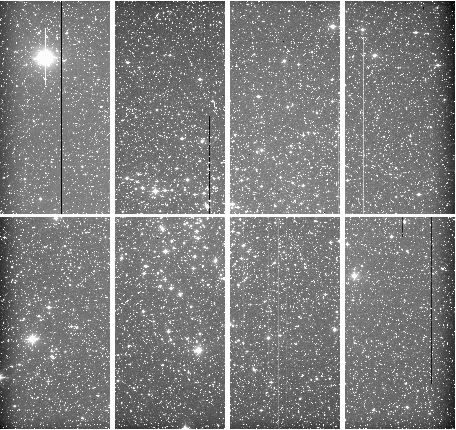
\includegraphics[width = 4in]{mosaicoBVineta.png}
\end{figure}

\begin{figure}[H]
  \centering
   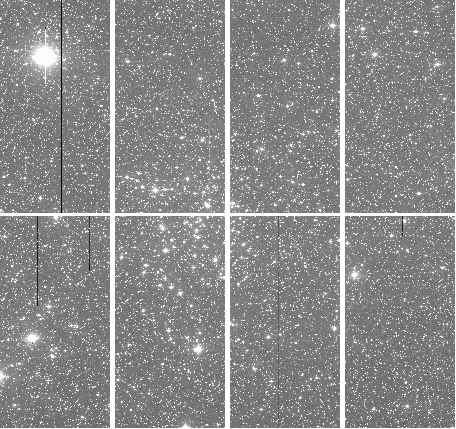
\includegraphics[width = 4in]{mosaicoB.png}
\end{figure}

A cada imagen reducida se le realizó el siguiente proceso:
\begin{itemize}
\item Usando DS9, se concluyó que los chips de interés son el 2,3,6 y 7. Por lo tanto, se separó las imágenes ciencia y se le agregó al header de cada una \tqt{IMAGETYP=OBJECT}.
\item Usando IMEXAMINE se encontró un FWHM promedio y una desviación estándar promedio para las imagenes mosaico: FWHM promedio fue 4.20, la desviación promedio ($\sigma$ ) fue 10. Adicionalmente se tomó un número de conteos máximo de 63000, de forma que se excluyen las estrellas saturadas. Usando esos datos y la tarea DAOFIND se generó una lista de coordenadas para cada chip.
\item Usando la lista de coordenadas se corre PHOT tal cual como se ha hecho en ejercicios pasados. Los datos de cada chip ya están incluidos en el header y se leen sin problema gracias a ESOSETINST. 
\item Se define un radio para el anillo de cielo y el radio de apertura. En este caso, dada la cercanía de algunas estrellas, se toma de radio de apertura 9 pixeles, de radio interior para el anillo de cielo 10 pixeles y de grosor para el anillo de cielo se tomó 10 pixeles.
\item Se usa TXDUMP para seleccionar seleccionar las columnas correctas para ejecutar DAOMATCH y DAOMASTER. Así mismo, se elimina las líneas con INDEF usando el programa de unix \tqt{grep}. Esto se hace con el comando:
\begin{lstlisting}[language=bash]
ecl> txdump imagen.mag.1 id,xcenter,ycenter,mag,merr yes |
grep -v INDEF > imagen.out
\end{lstlisting}
\item Ya con los archivos \tqt{.out} de cada imagen ciencia, utilizamos DAOMATCH y DAOMASTER de a parejas de archivos. Primero se elije el archivo master (se toma el que tenga más estrellas), luego se ejecuta DAOMATCH y la primera entrada correspondería al archivo master, la segunda a la otra imagen ciencia de interés. Por ejemplo, para un diagrama B-V, se tomaría V como master (tiene más imagenes) y B sería la segunda entrada. 
\item De la ejecución \emph{exitosa} de DAOMATCH, se obtiene un archivo \tqt{.mch} con la transformacion de coordenadas entre los archivos. Se ejecuta DAOMASTER y se le pasa de entrada el archivo .mch. Se selecciona 6 grados de libertad y un número mínimo de frames de 2, una fracción mínima de 0.5 y un número de recuadros suficientes de 2. Estos valores corresponden a los mismos utilizados en el ejercicio de DAOMATCH y DAOMASTER con M92.
\item De correr exitosamente DAOMASTER se obtiene un archivo \tqt{.raw} con la lista de estrellas detectadas en ambas imágenes, junto a sus coordenadas y magnitudes en las bandas de interés. Escribiendo un script de python, se genera el diagrama magnitud color para cada chip tanto en B-V como V-Rc. Por último, se genera un diagrama para todos los chips en B-V y un diagrama para todos los chips en V-Rc.
\end{itemize}

\section{Resultados}
A continuación se presentan los diagrama color magnitud obtenidos para los diferentes chips. 
\begin{figure}[H]
  \centering
   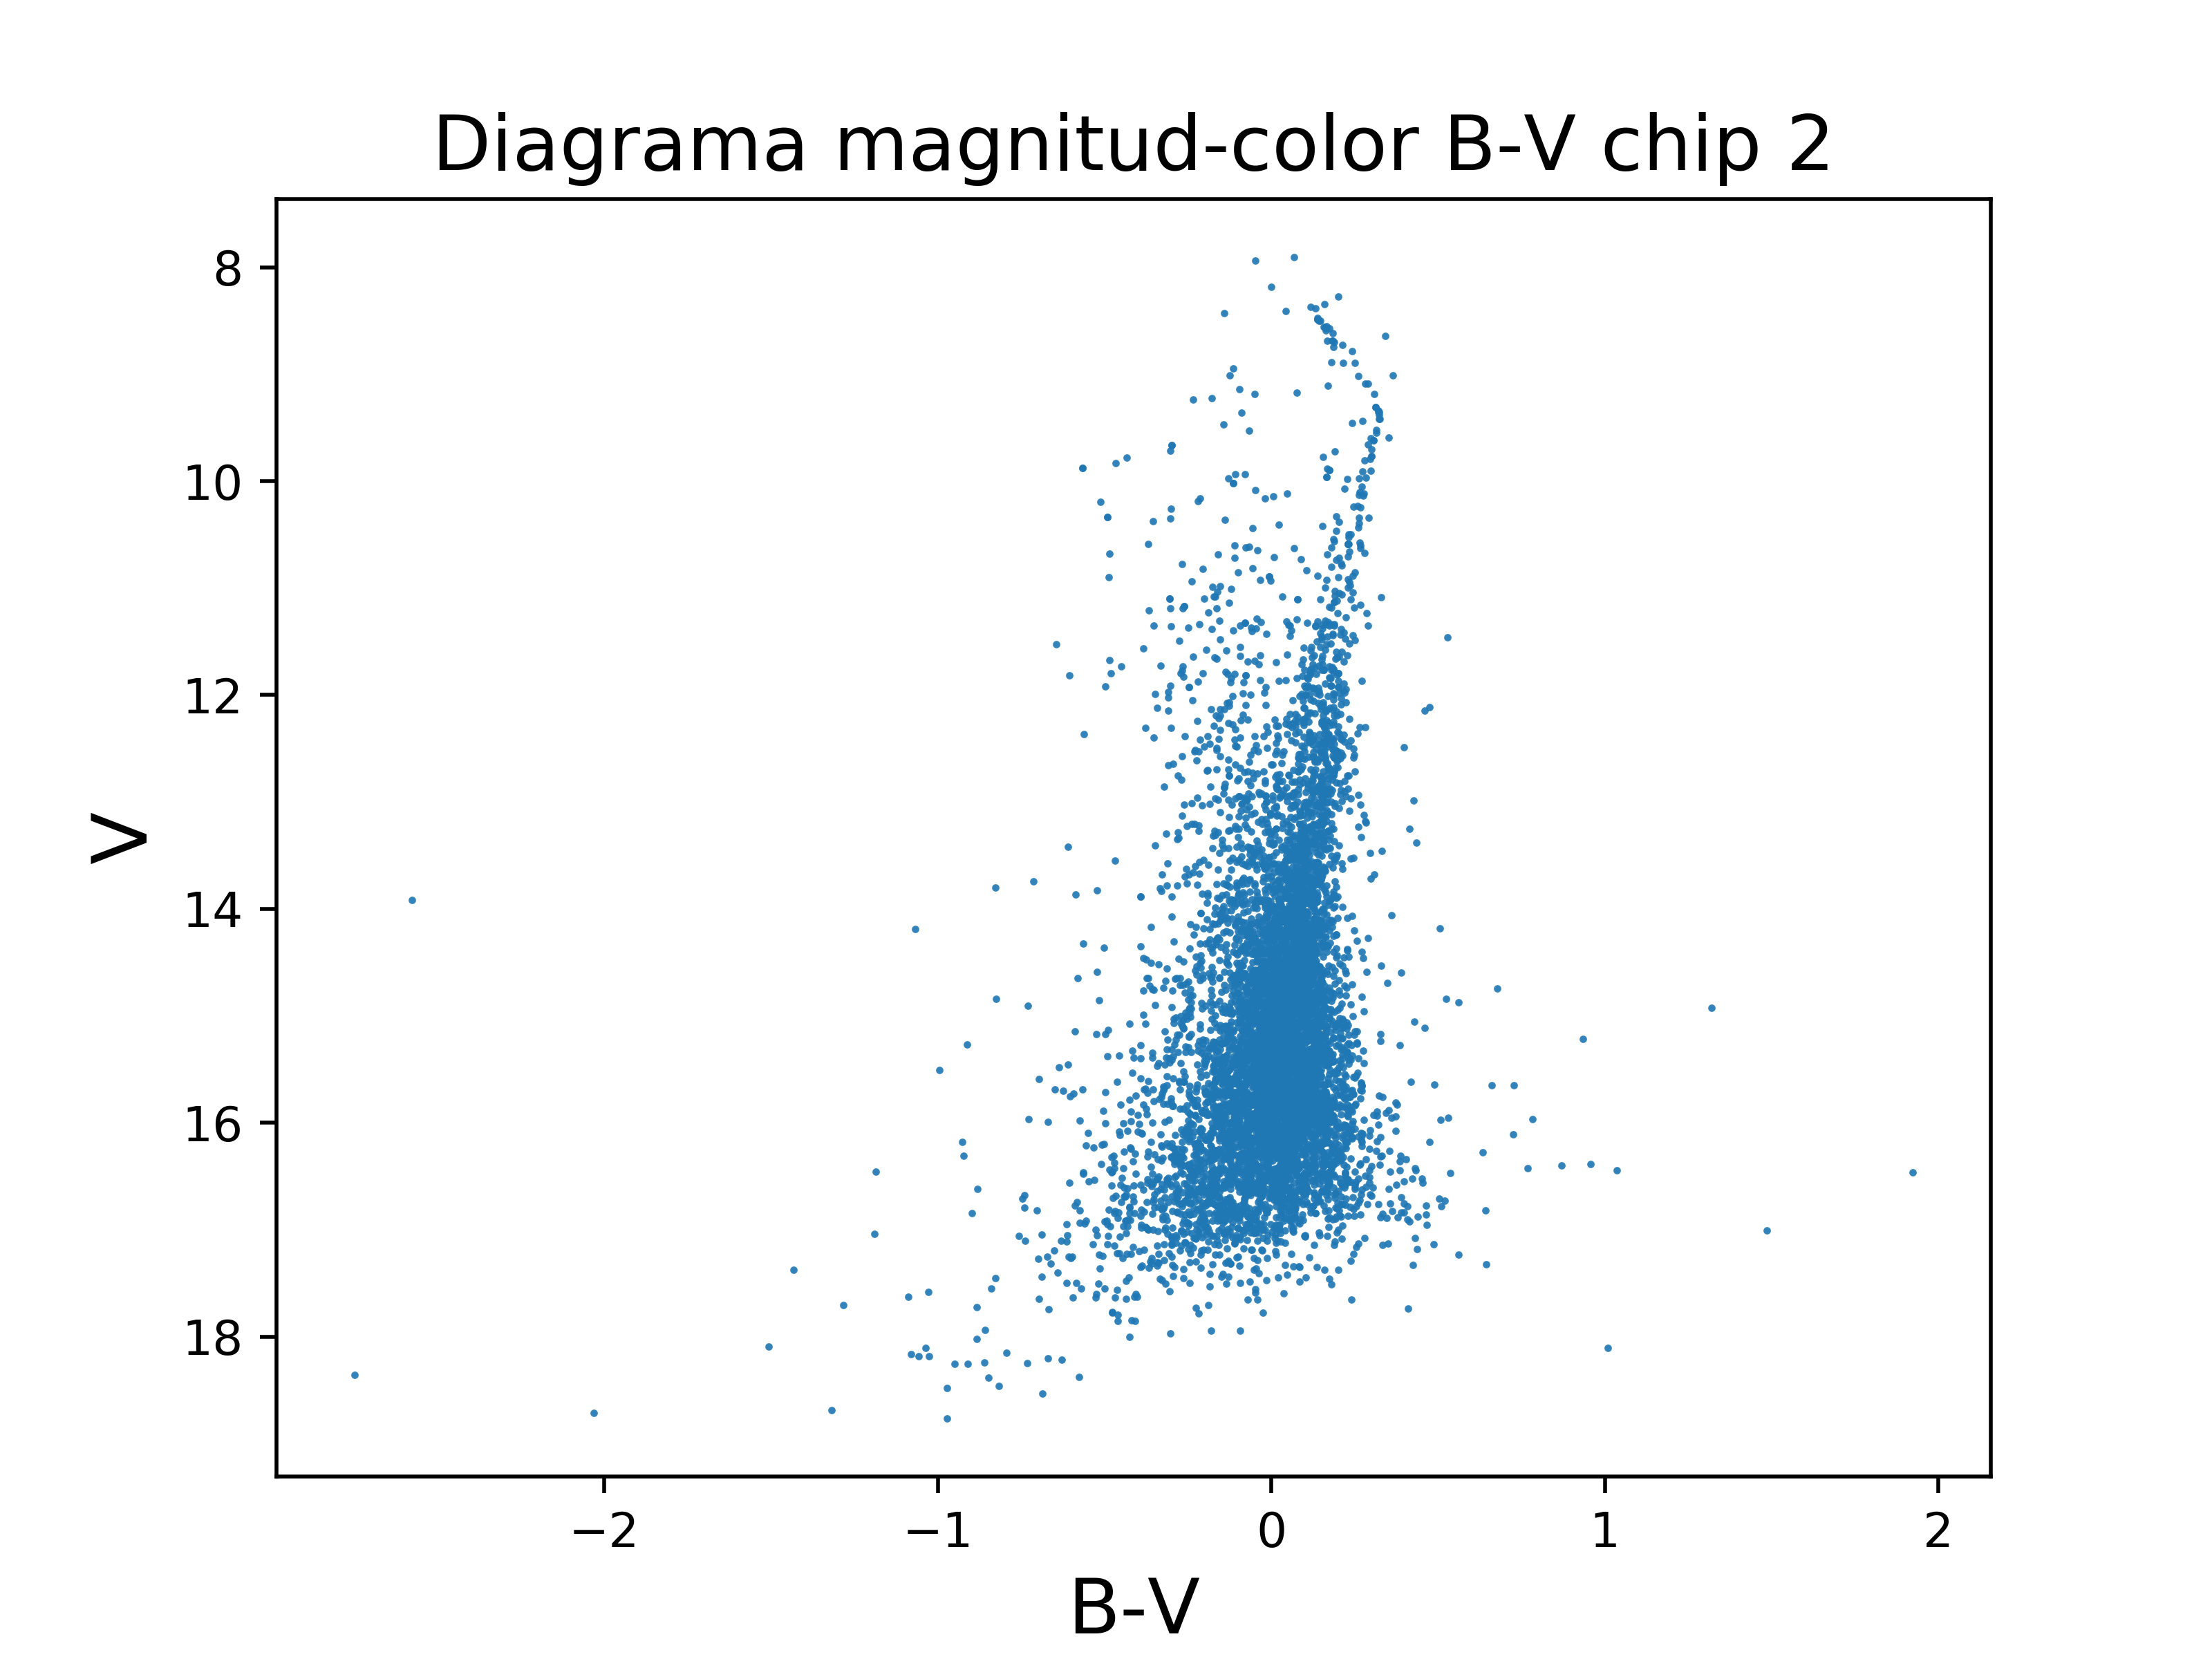
\includegraphics[width = 4in]{B-V2.png}
\end{figure}
\begin{figure}[H]
  \centering
   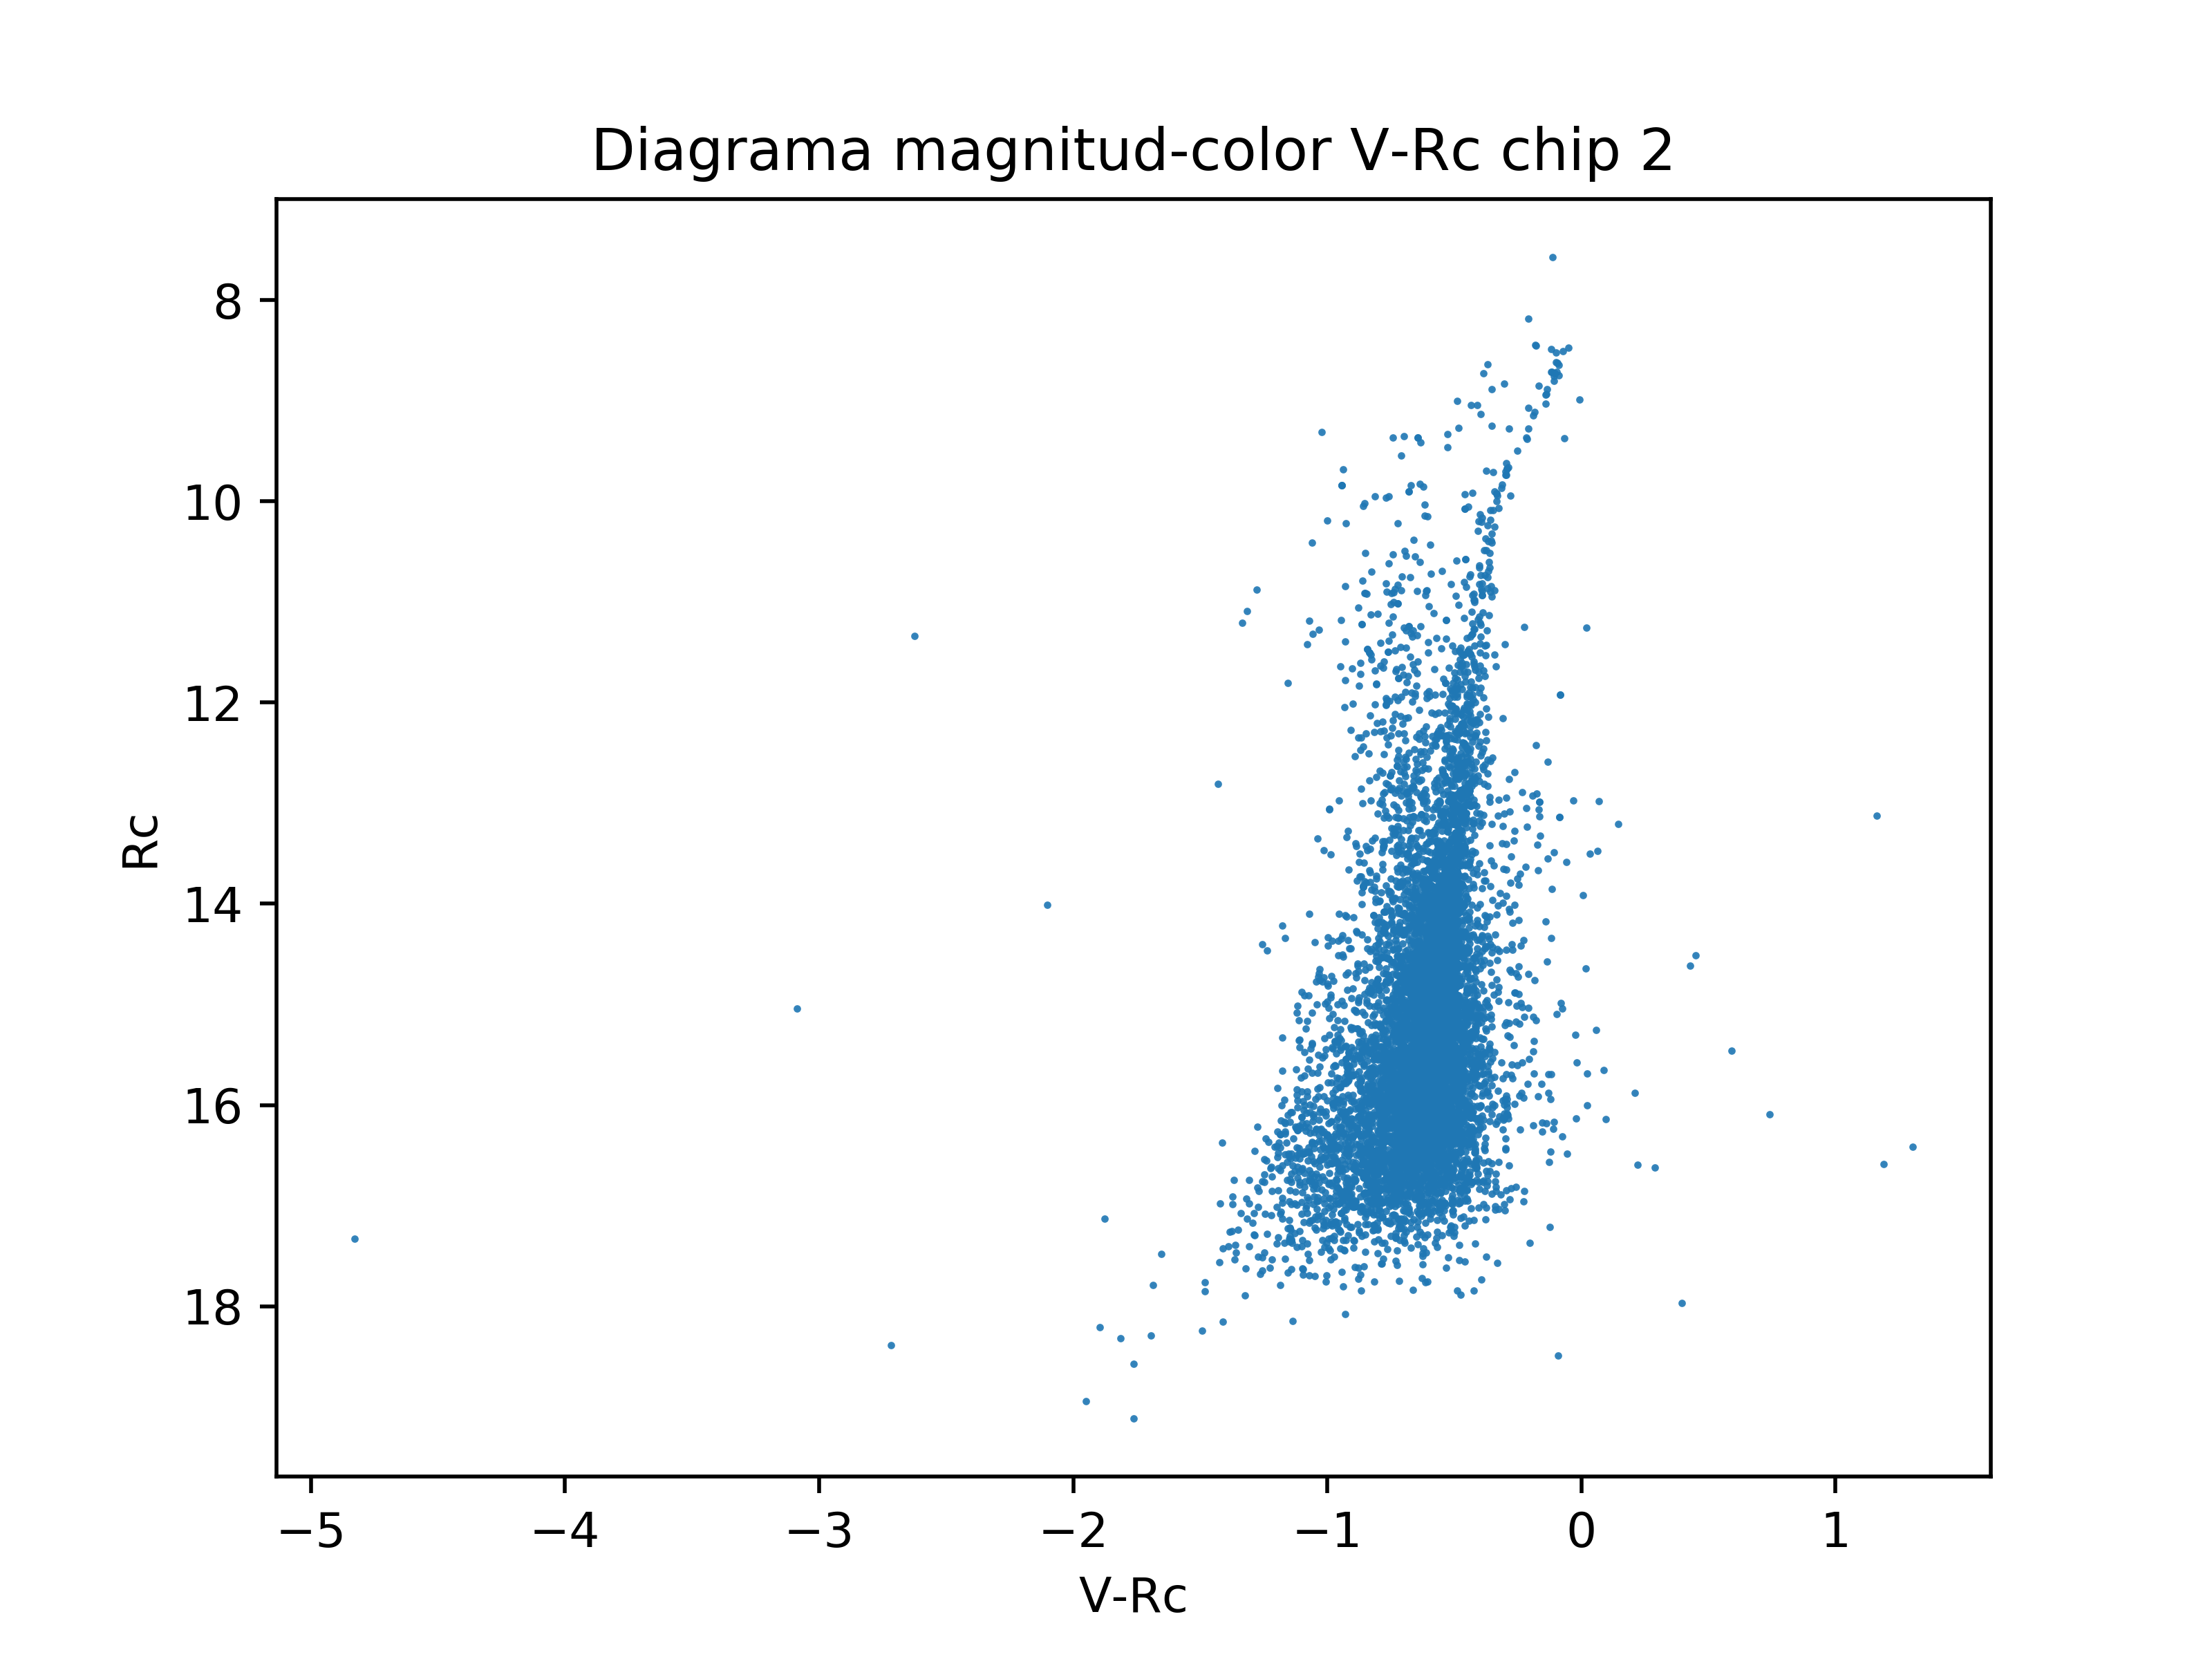
\includegraphics[width = 4in]{V-Rc2.png}
\end{figure}

\begin{figure}[H]
  \centering
   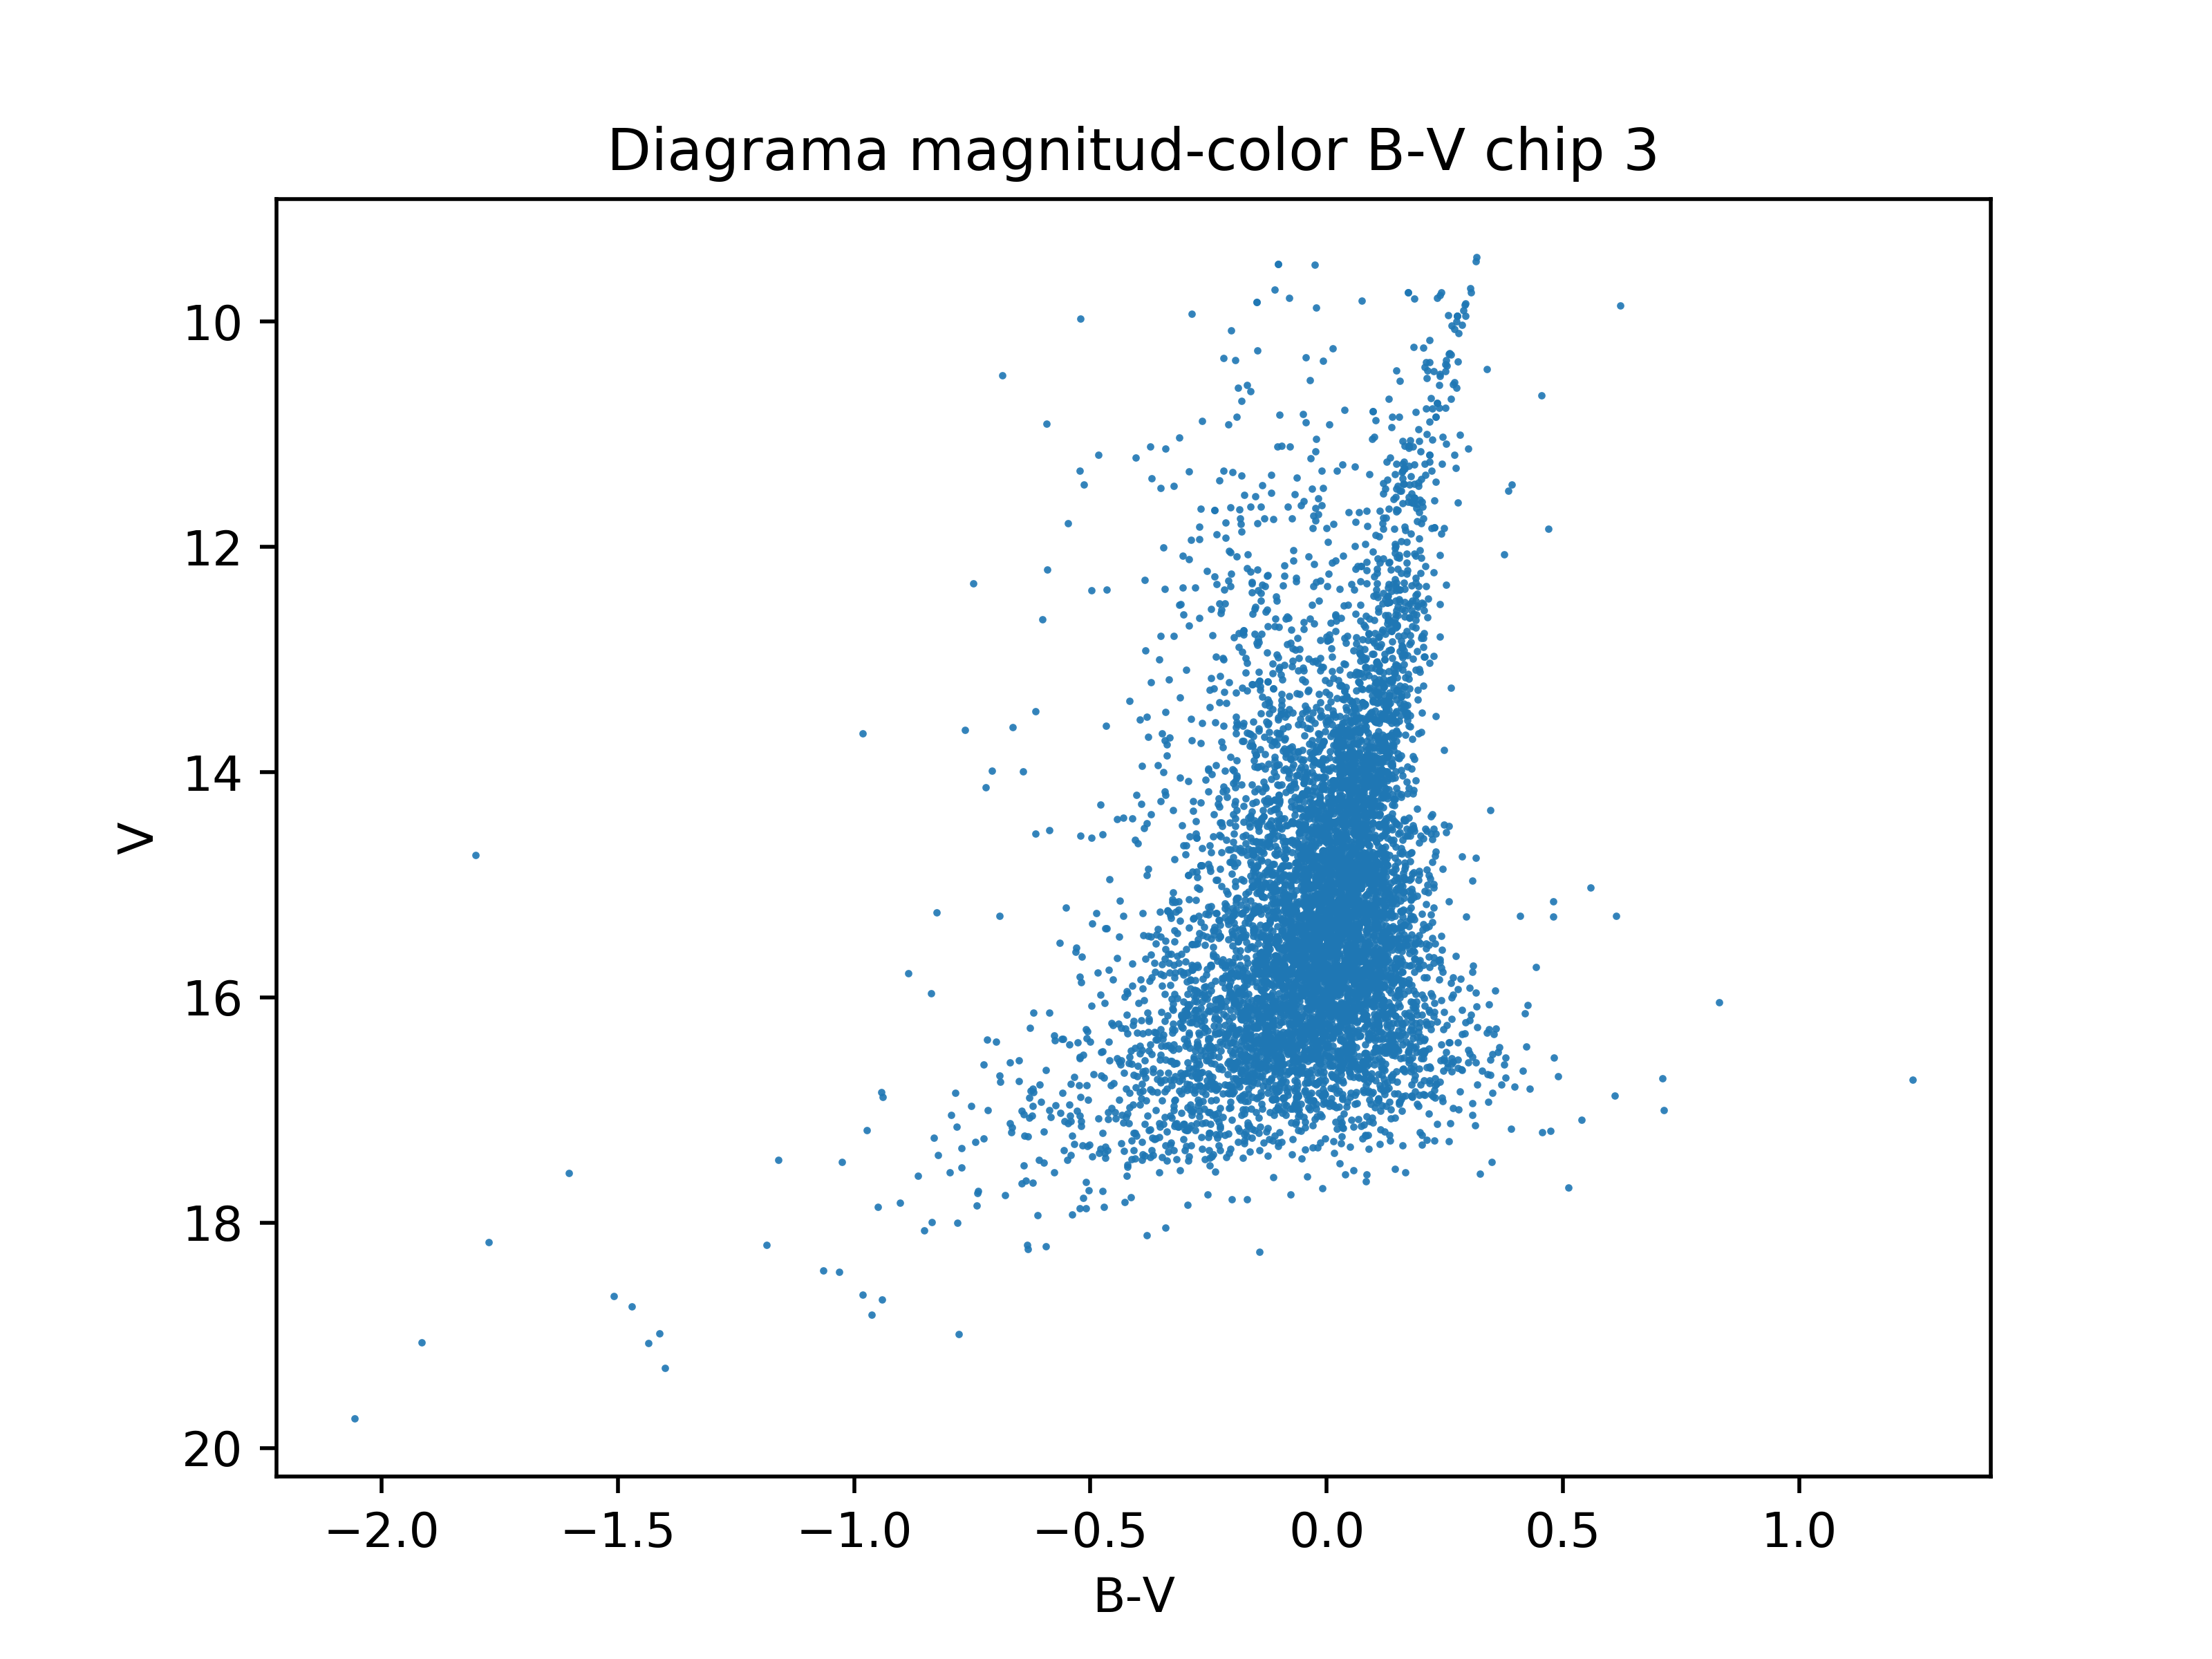
\includegraphics[width = 4in]{B-V3.png}
\end{figure}
\begin{figure}[H]
  \centering
   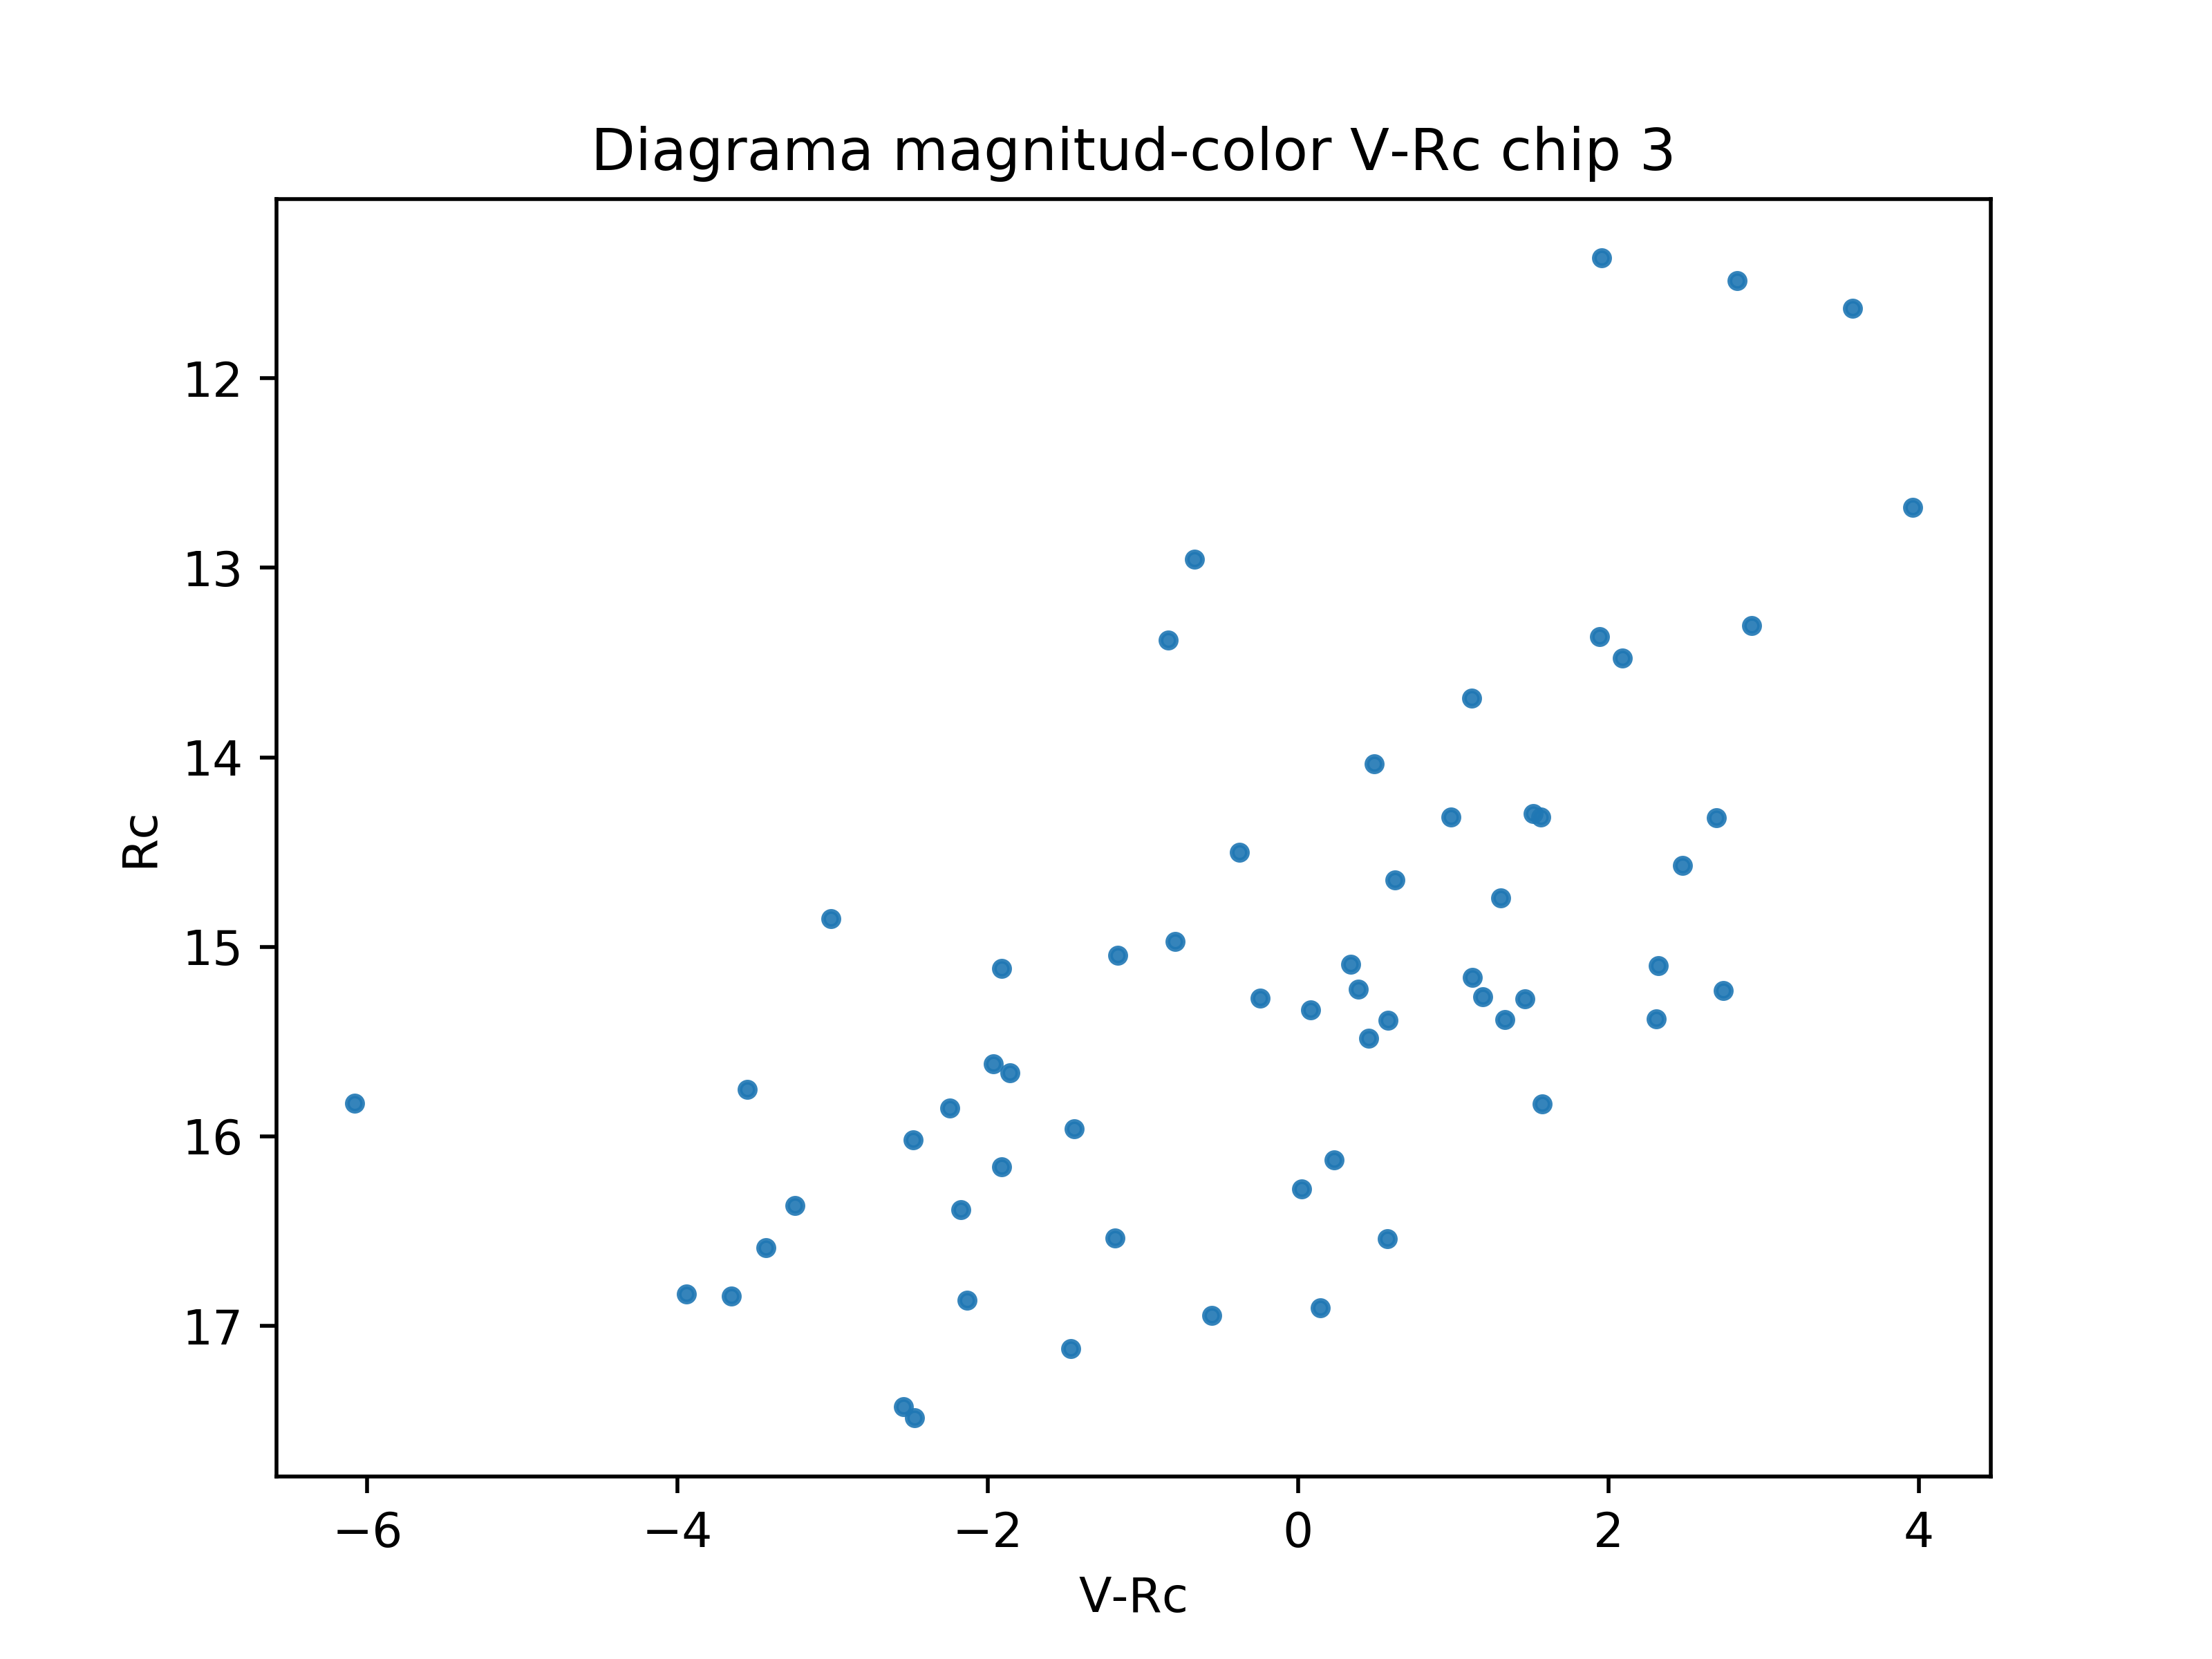
\includegraphics[width = 4in]{V-Rc3.png}
\end{figure}

\begin{figure}[H]
  \centering
   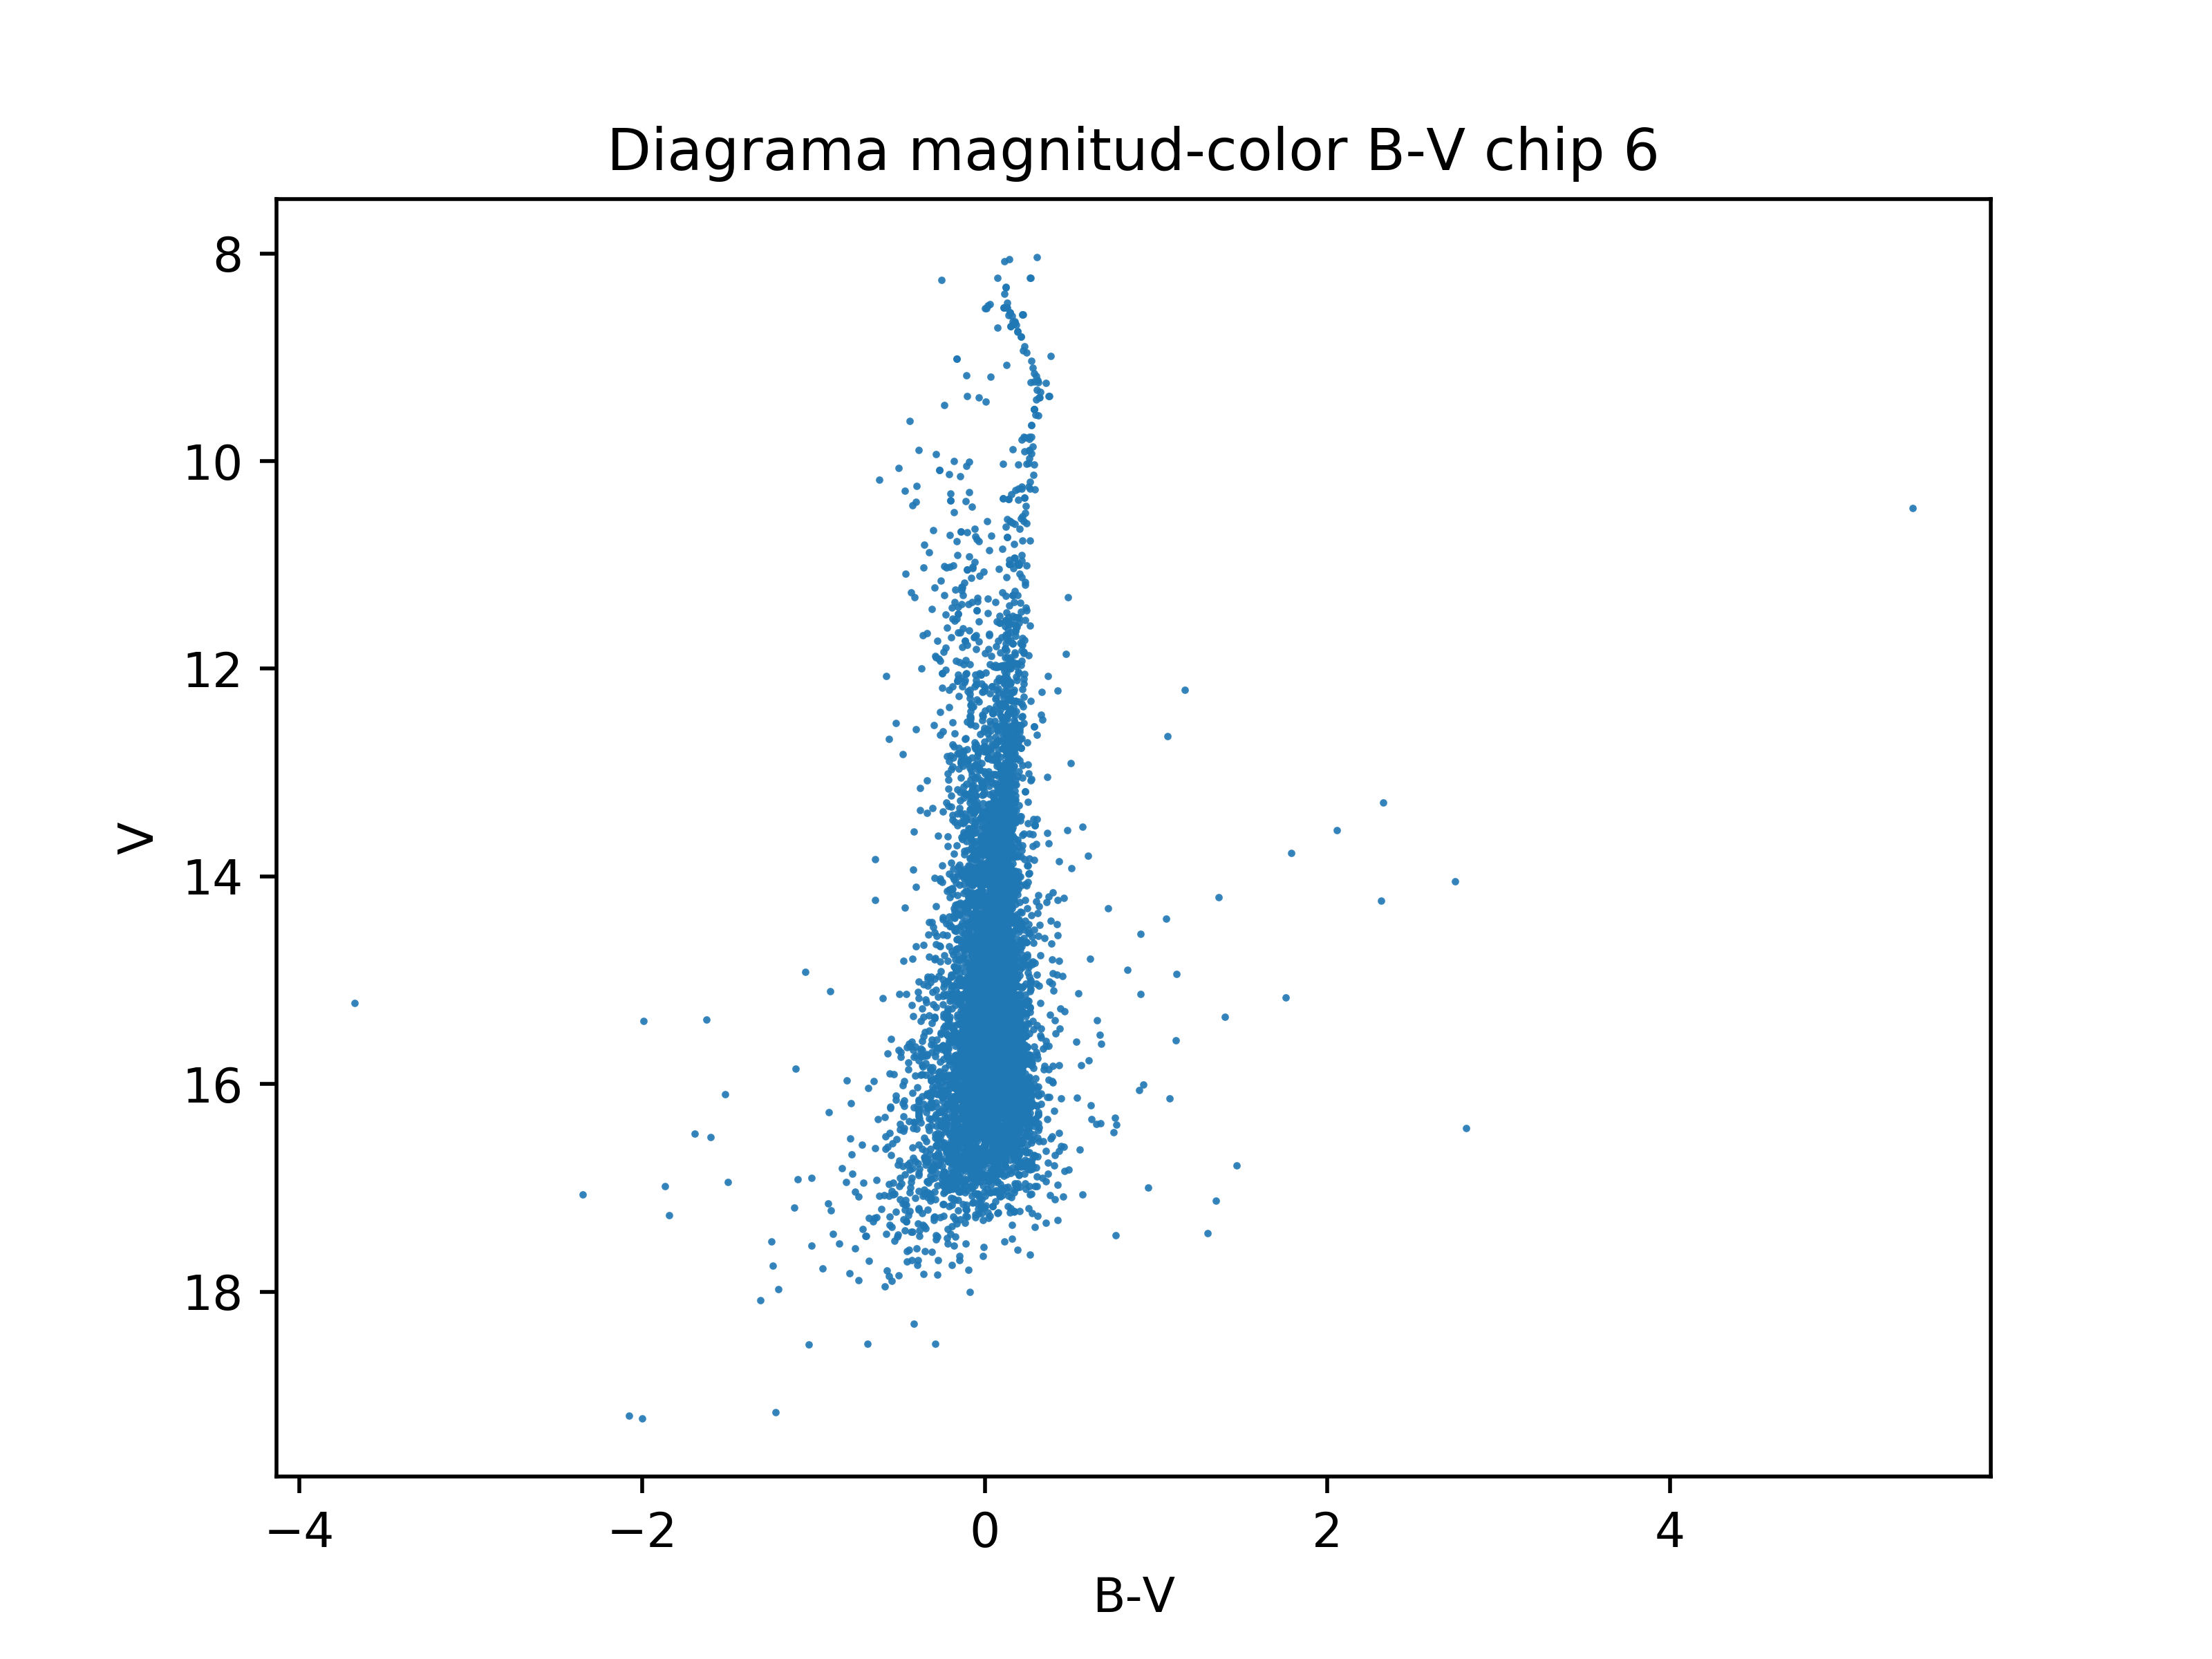
\includegraphics[width = 4in]{B-V6.png}
\end{figure}
\begin{figure}[H]
  \centering
   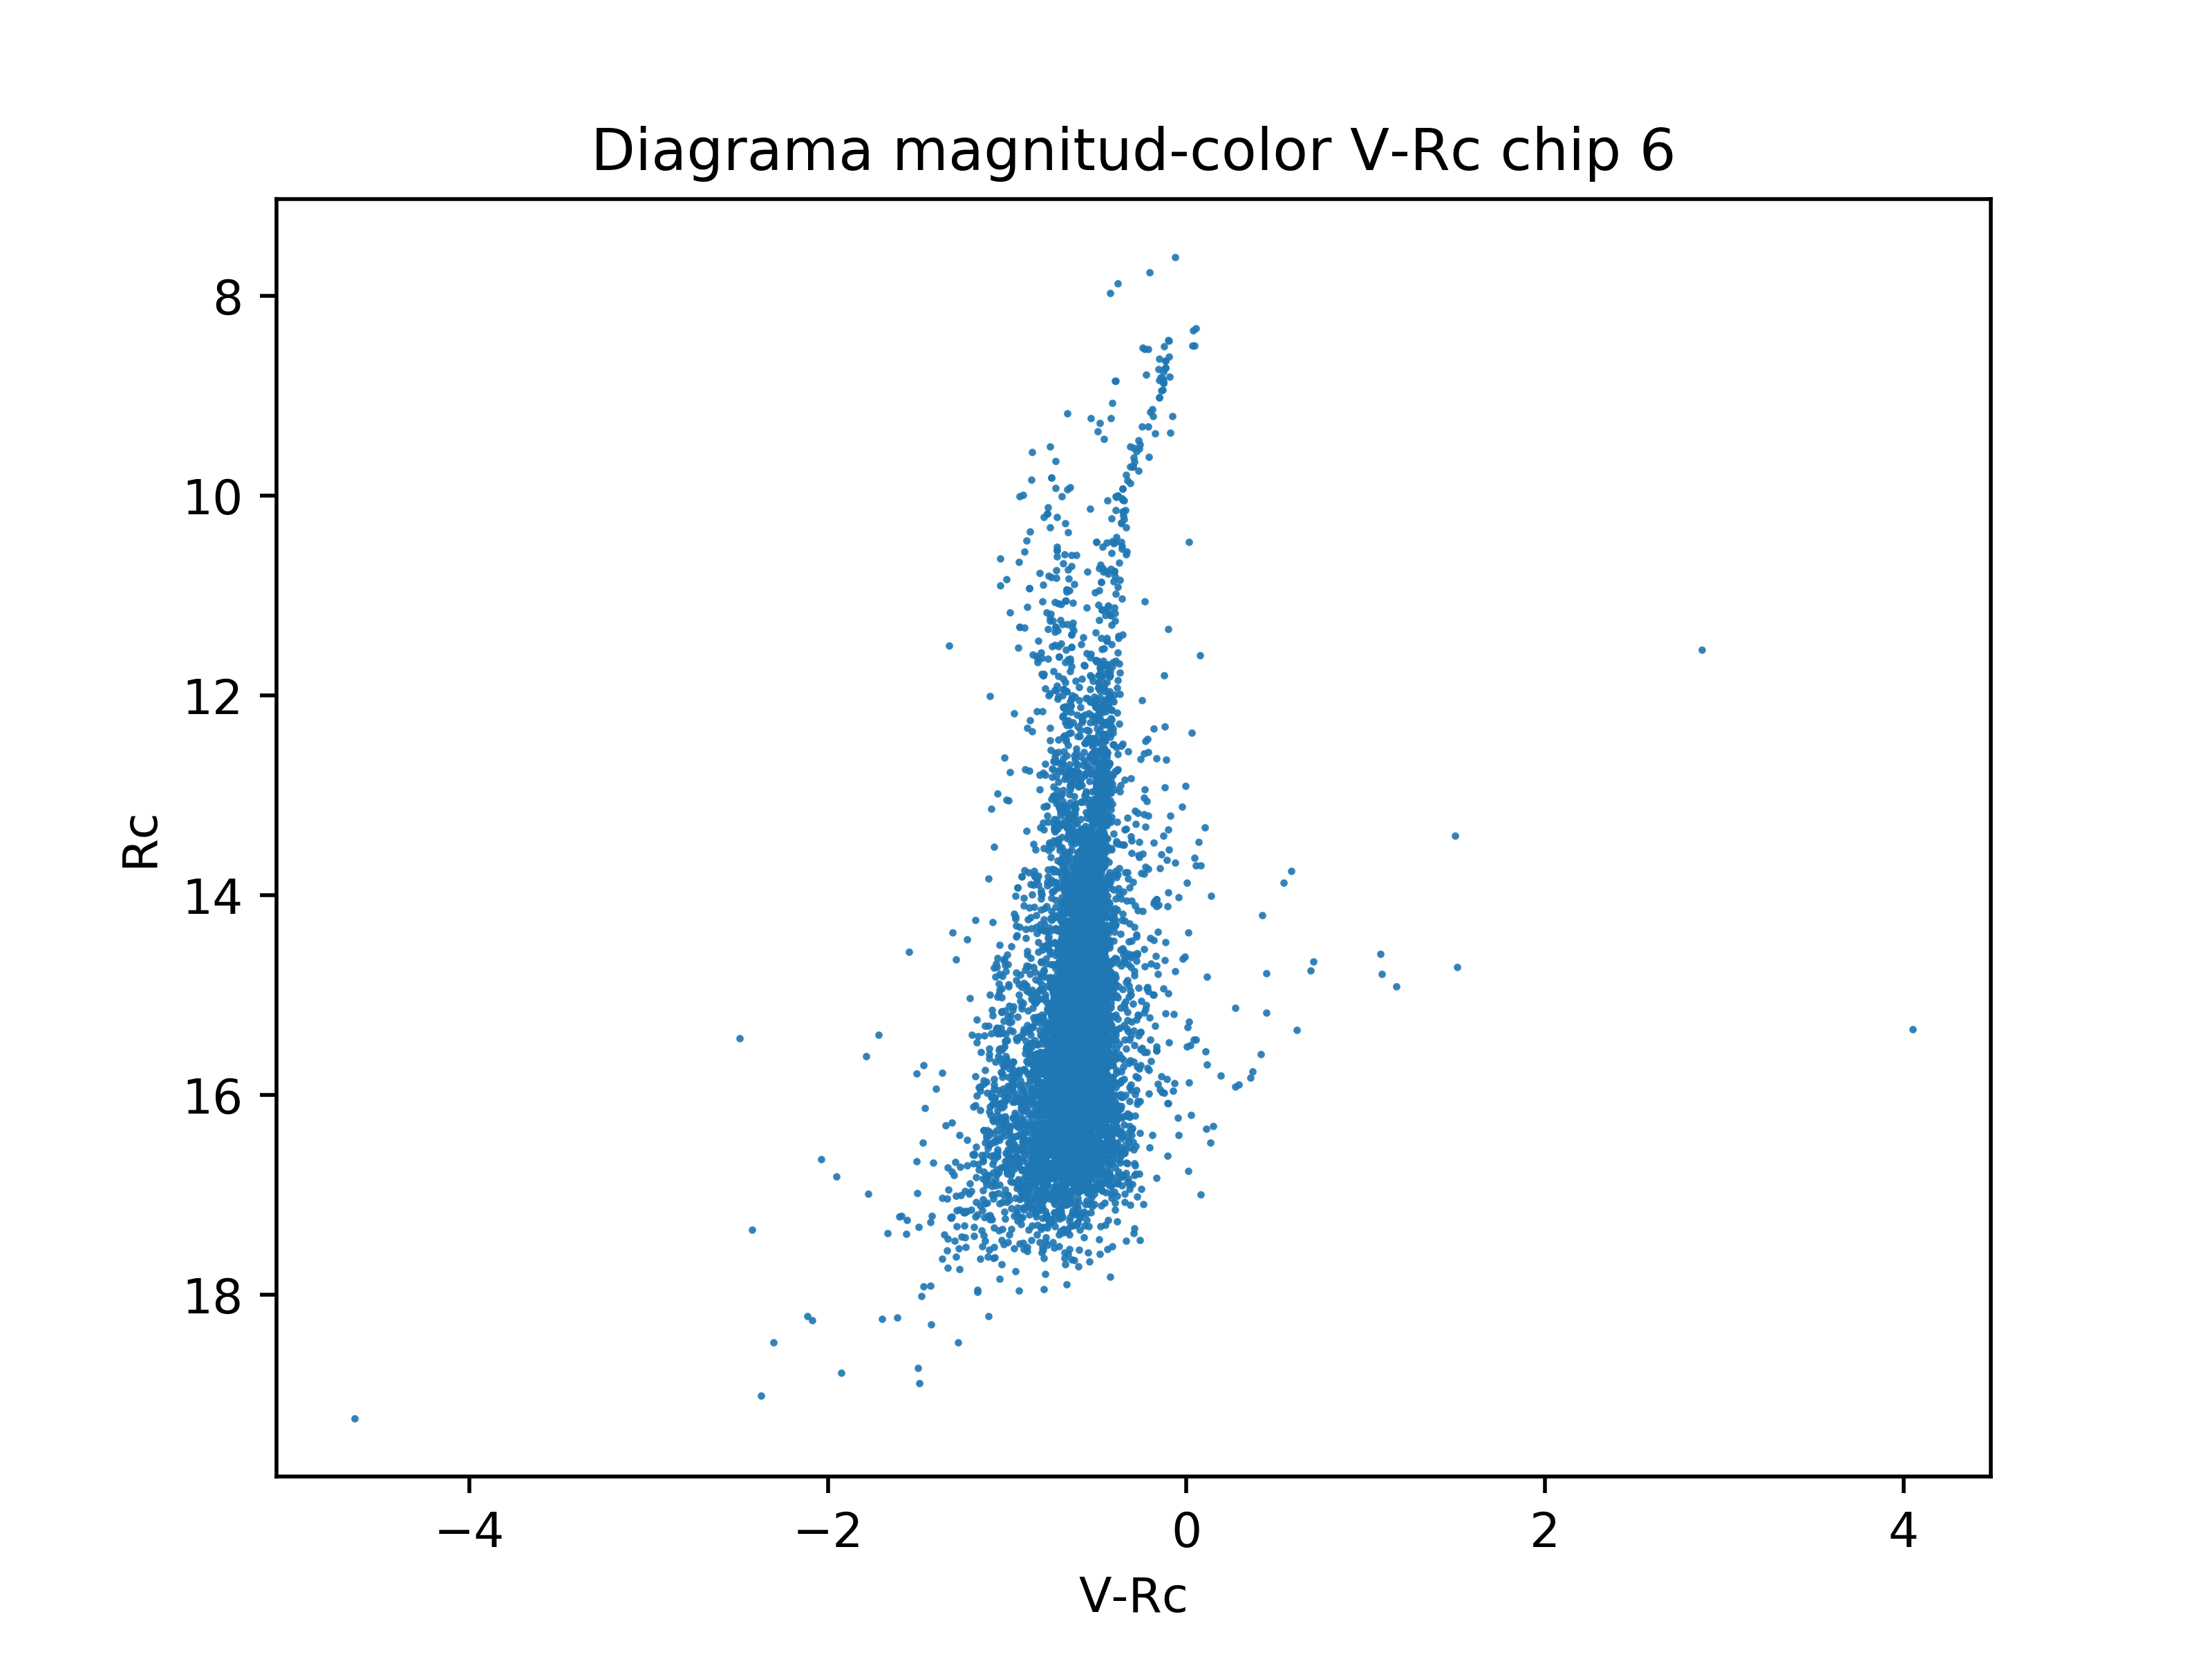
\includegraphics[width = 4in]{V-Rc6.png}
\end{figure}

\begin{figure}[H]
  \centering
   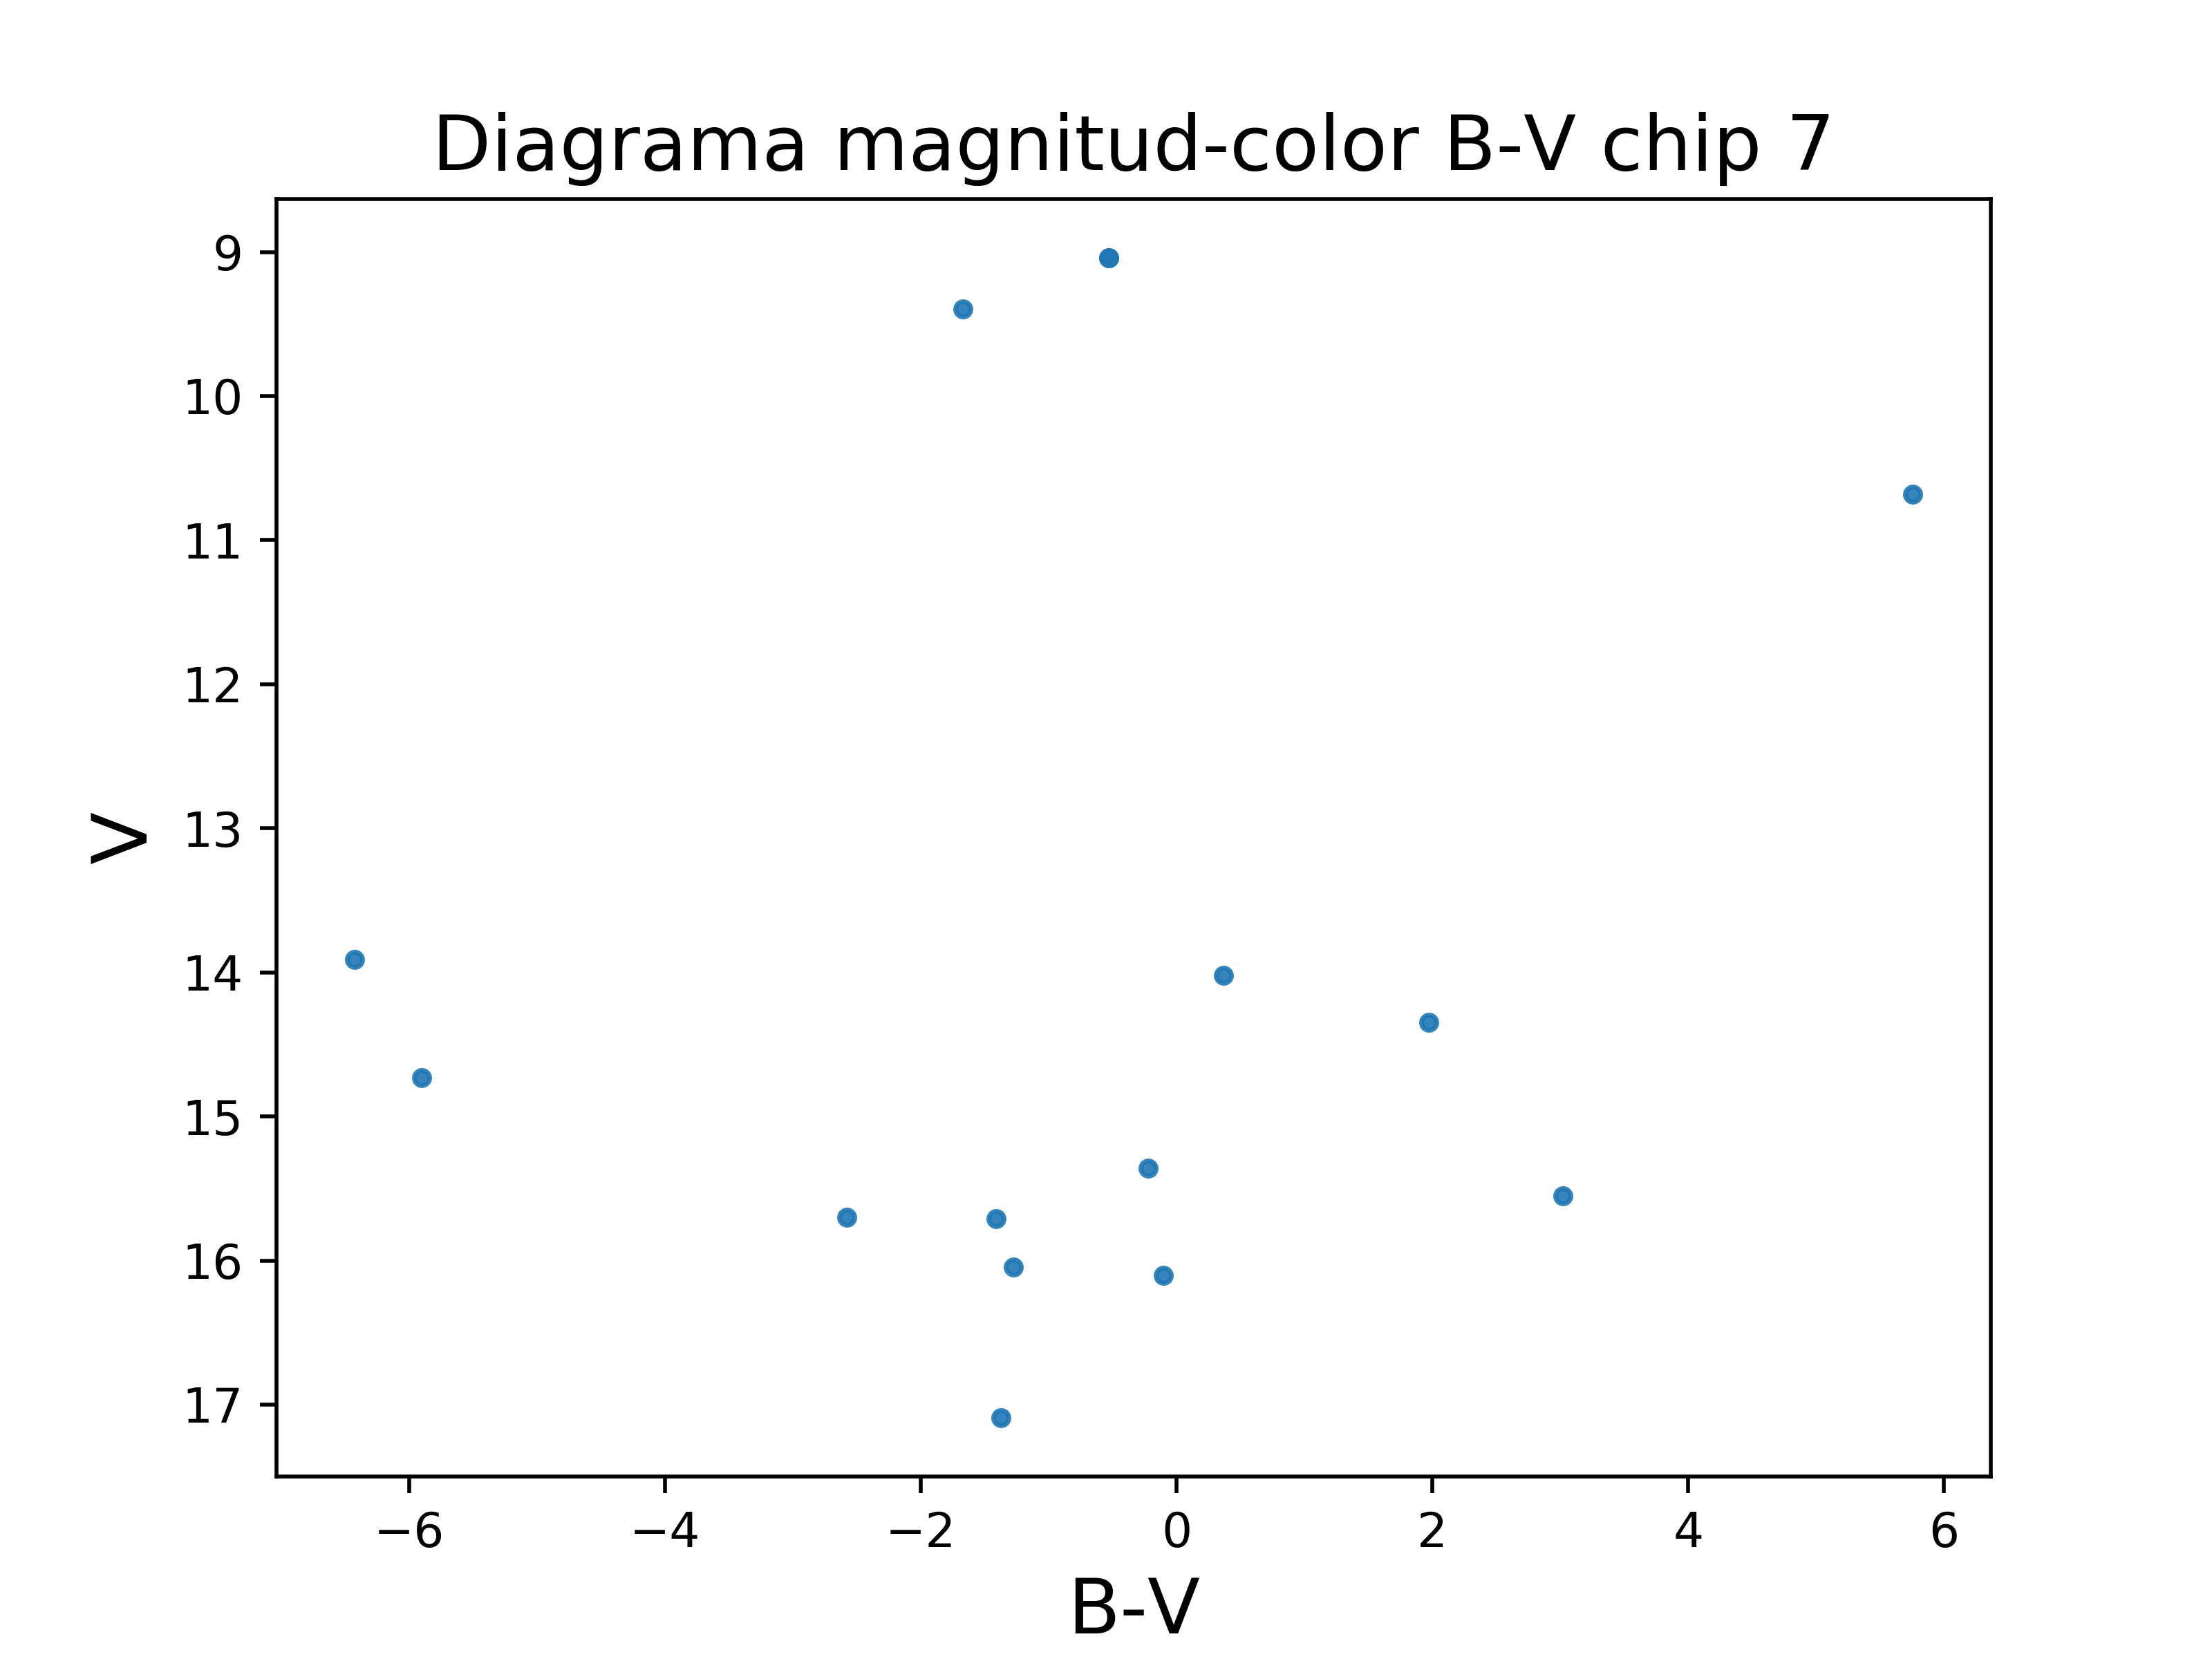
\includegraphics[width = 4in]{B-V7.png}
\end{figure}
\begin{figure}[H]
  \centering
   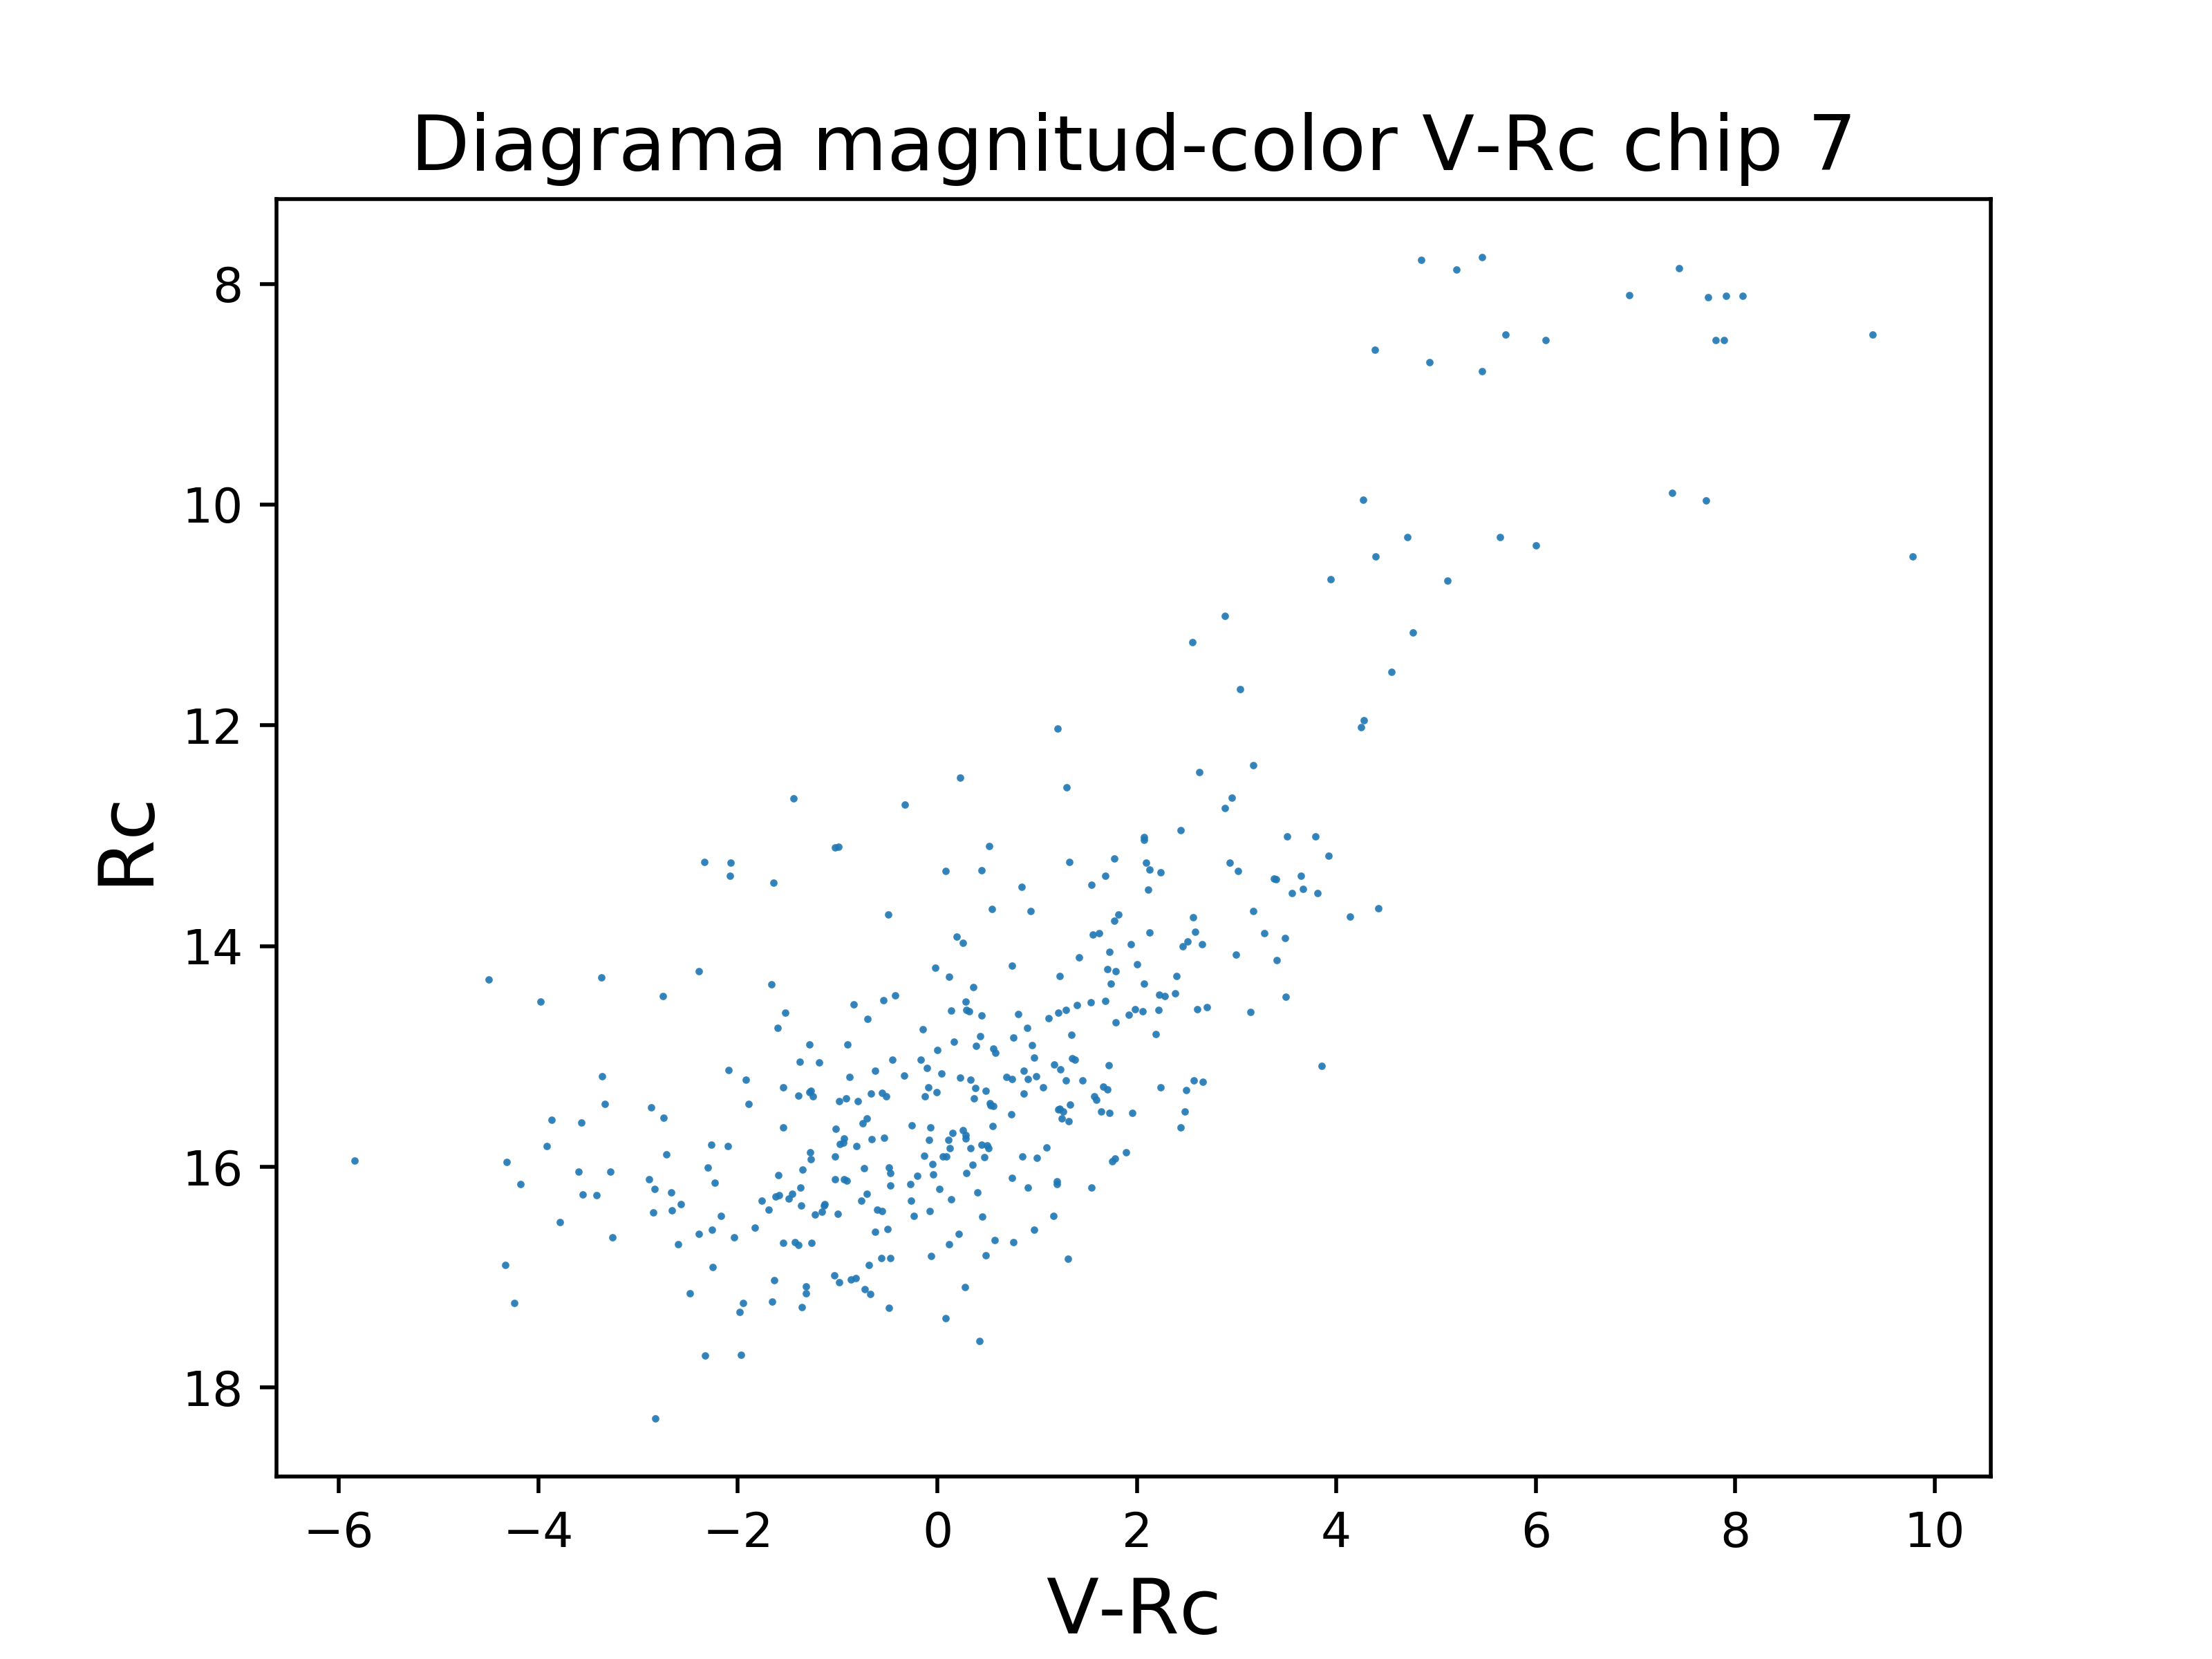
\includegraphics[width = 4in]{V-Rc7.png}
\end{figure}
   
  Se observa que para los chips 2 y 6 se logró relacionar un buen número de estrellas, sin embargo, para el chip 3 solo se encontró bastantes estrellas en el caso B-V. Para el chip 7 ningún caso logró encontrar un buen número de estrellas. Los problemas para relacionar estrellas entre los frames pueden deberse a los parámetros utilizados en la fotometría.

Finalmente, se presentan a continuación los diagramas magnitud-color de los chips de interés juntos:


\begin{figure}[H]
  \centering
   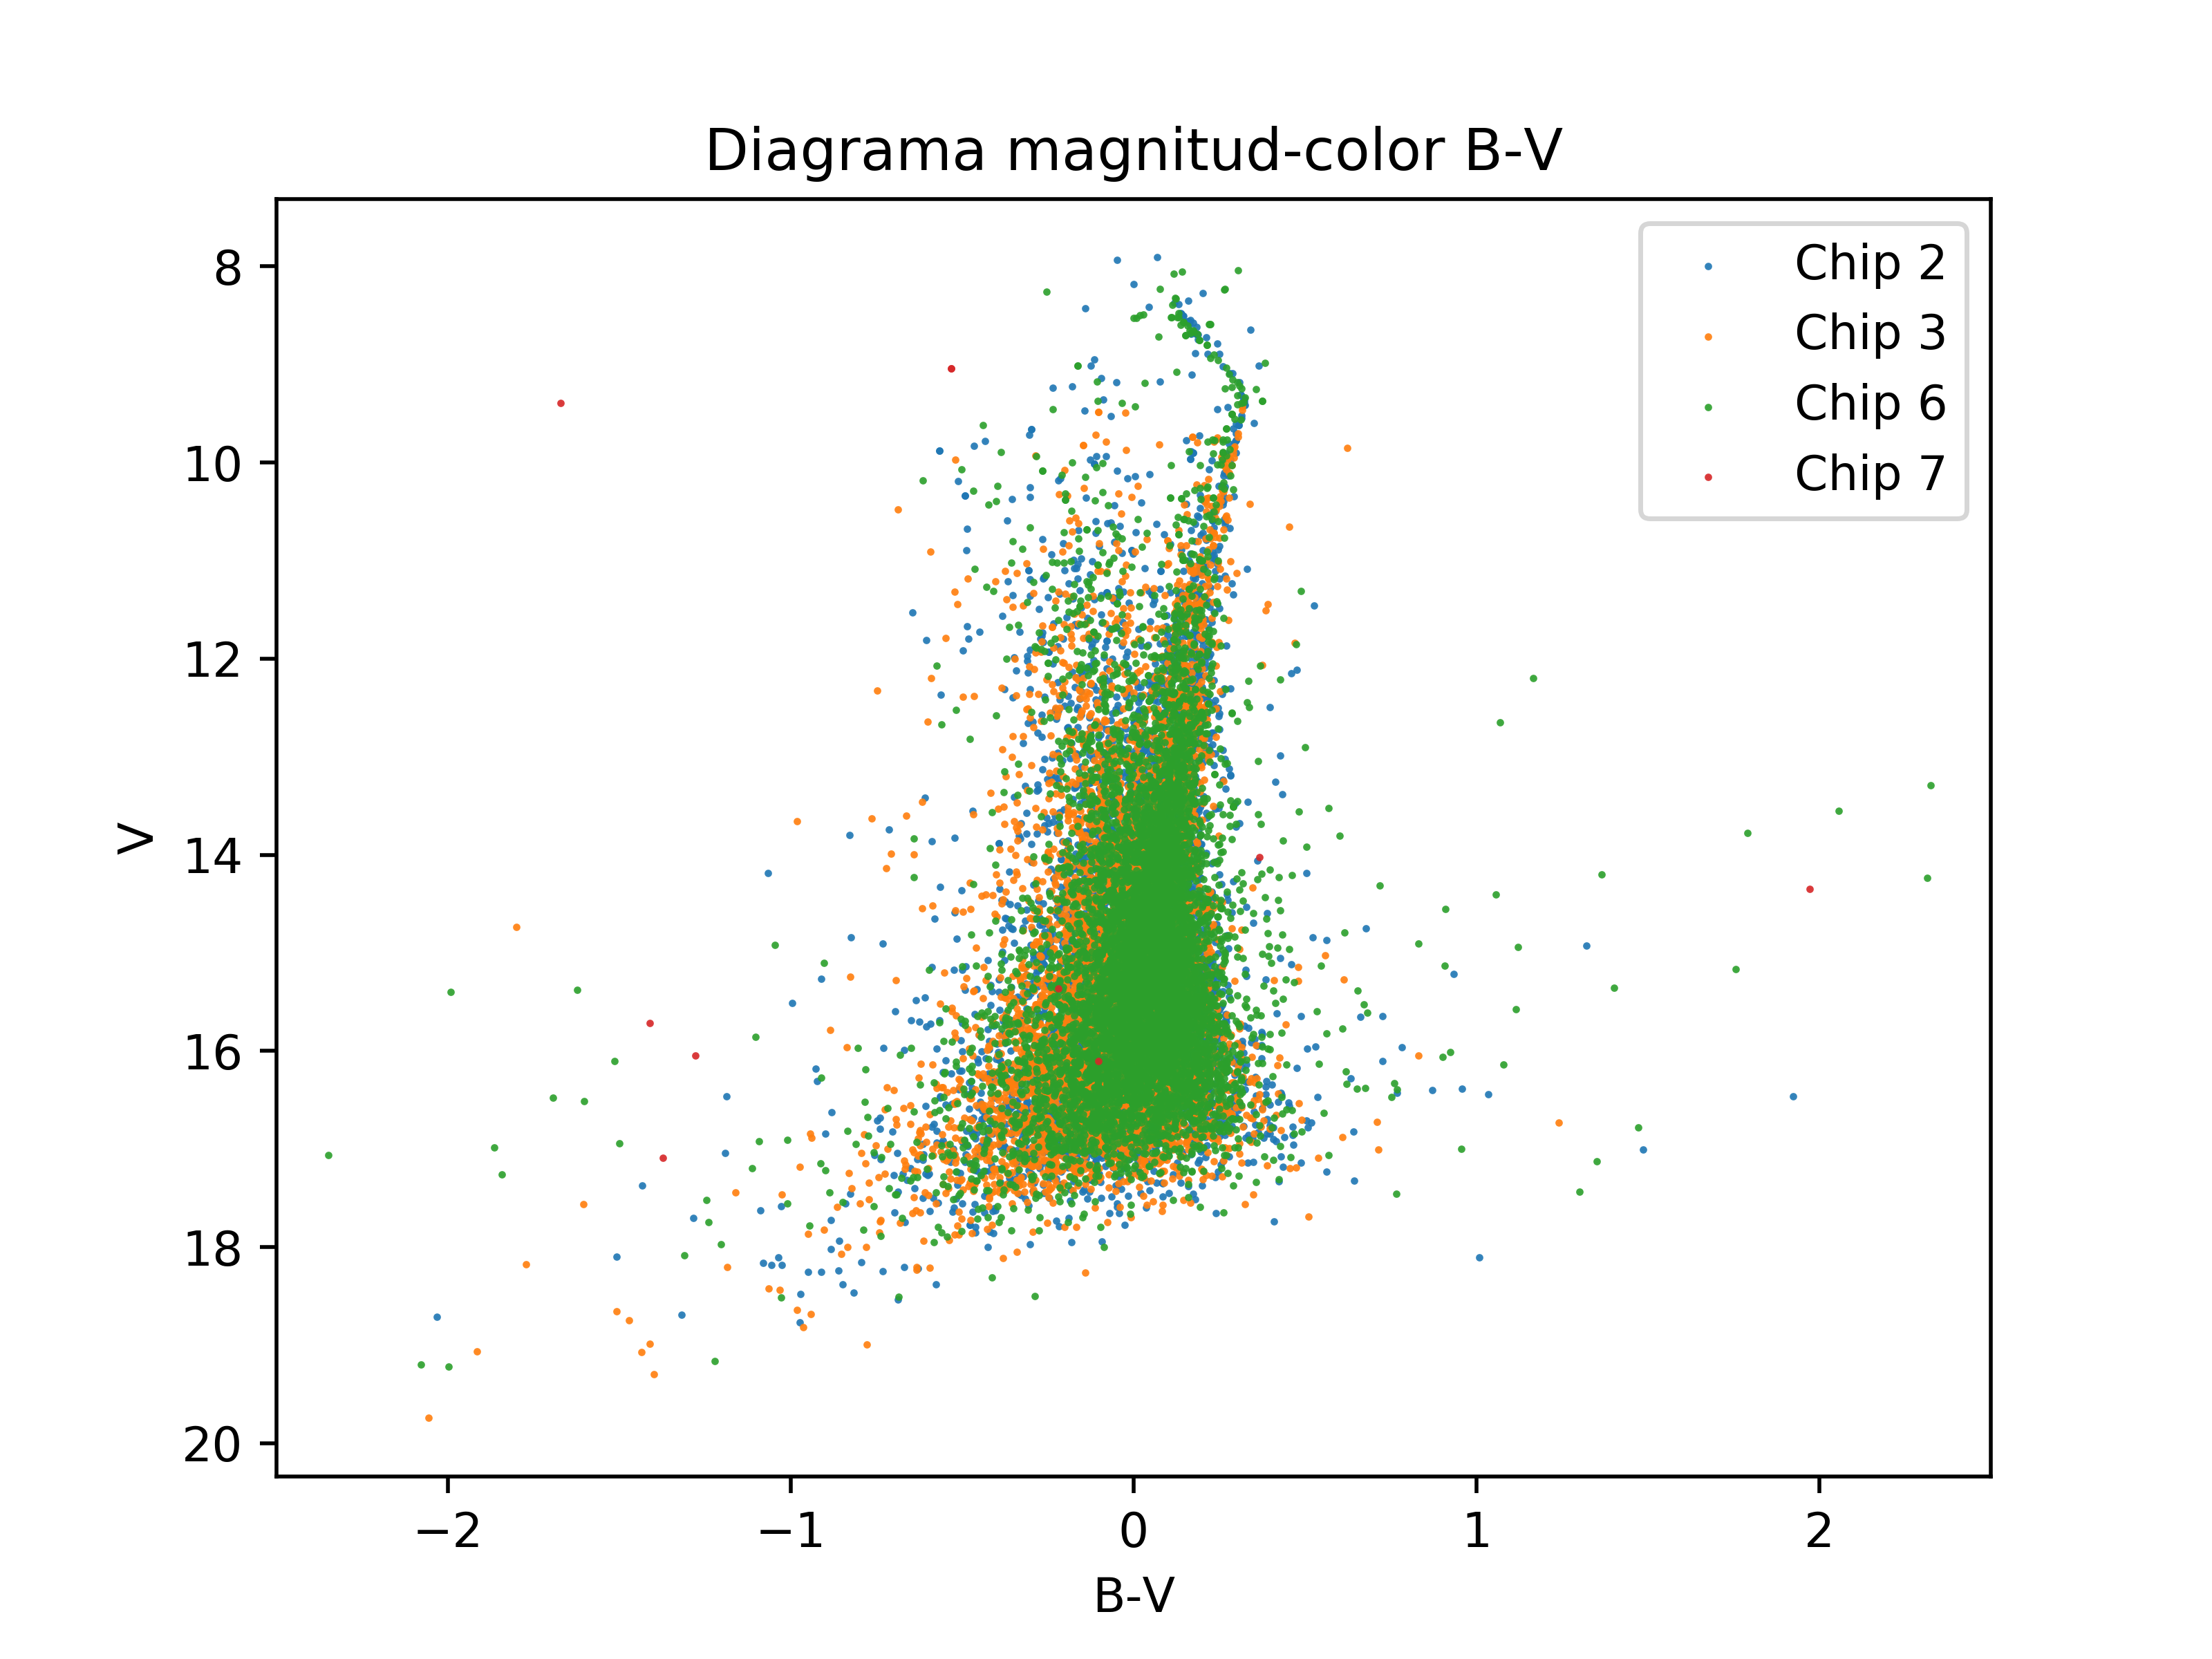
\includegraphics[width = 4in]{diagramaMagnitudColor.png}
\end{figure}
\begin{figure}[H]
  \centering
   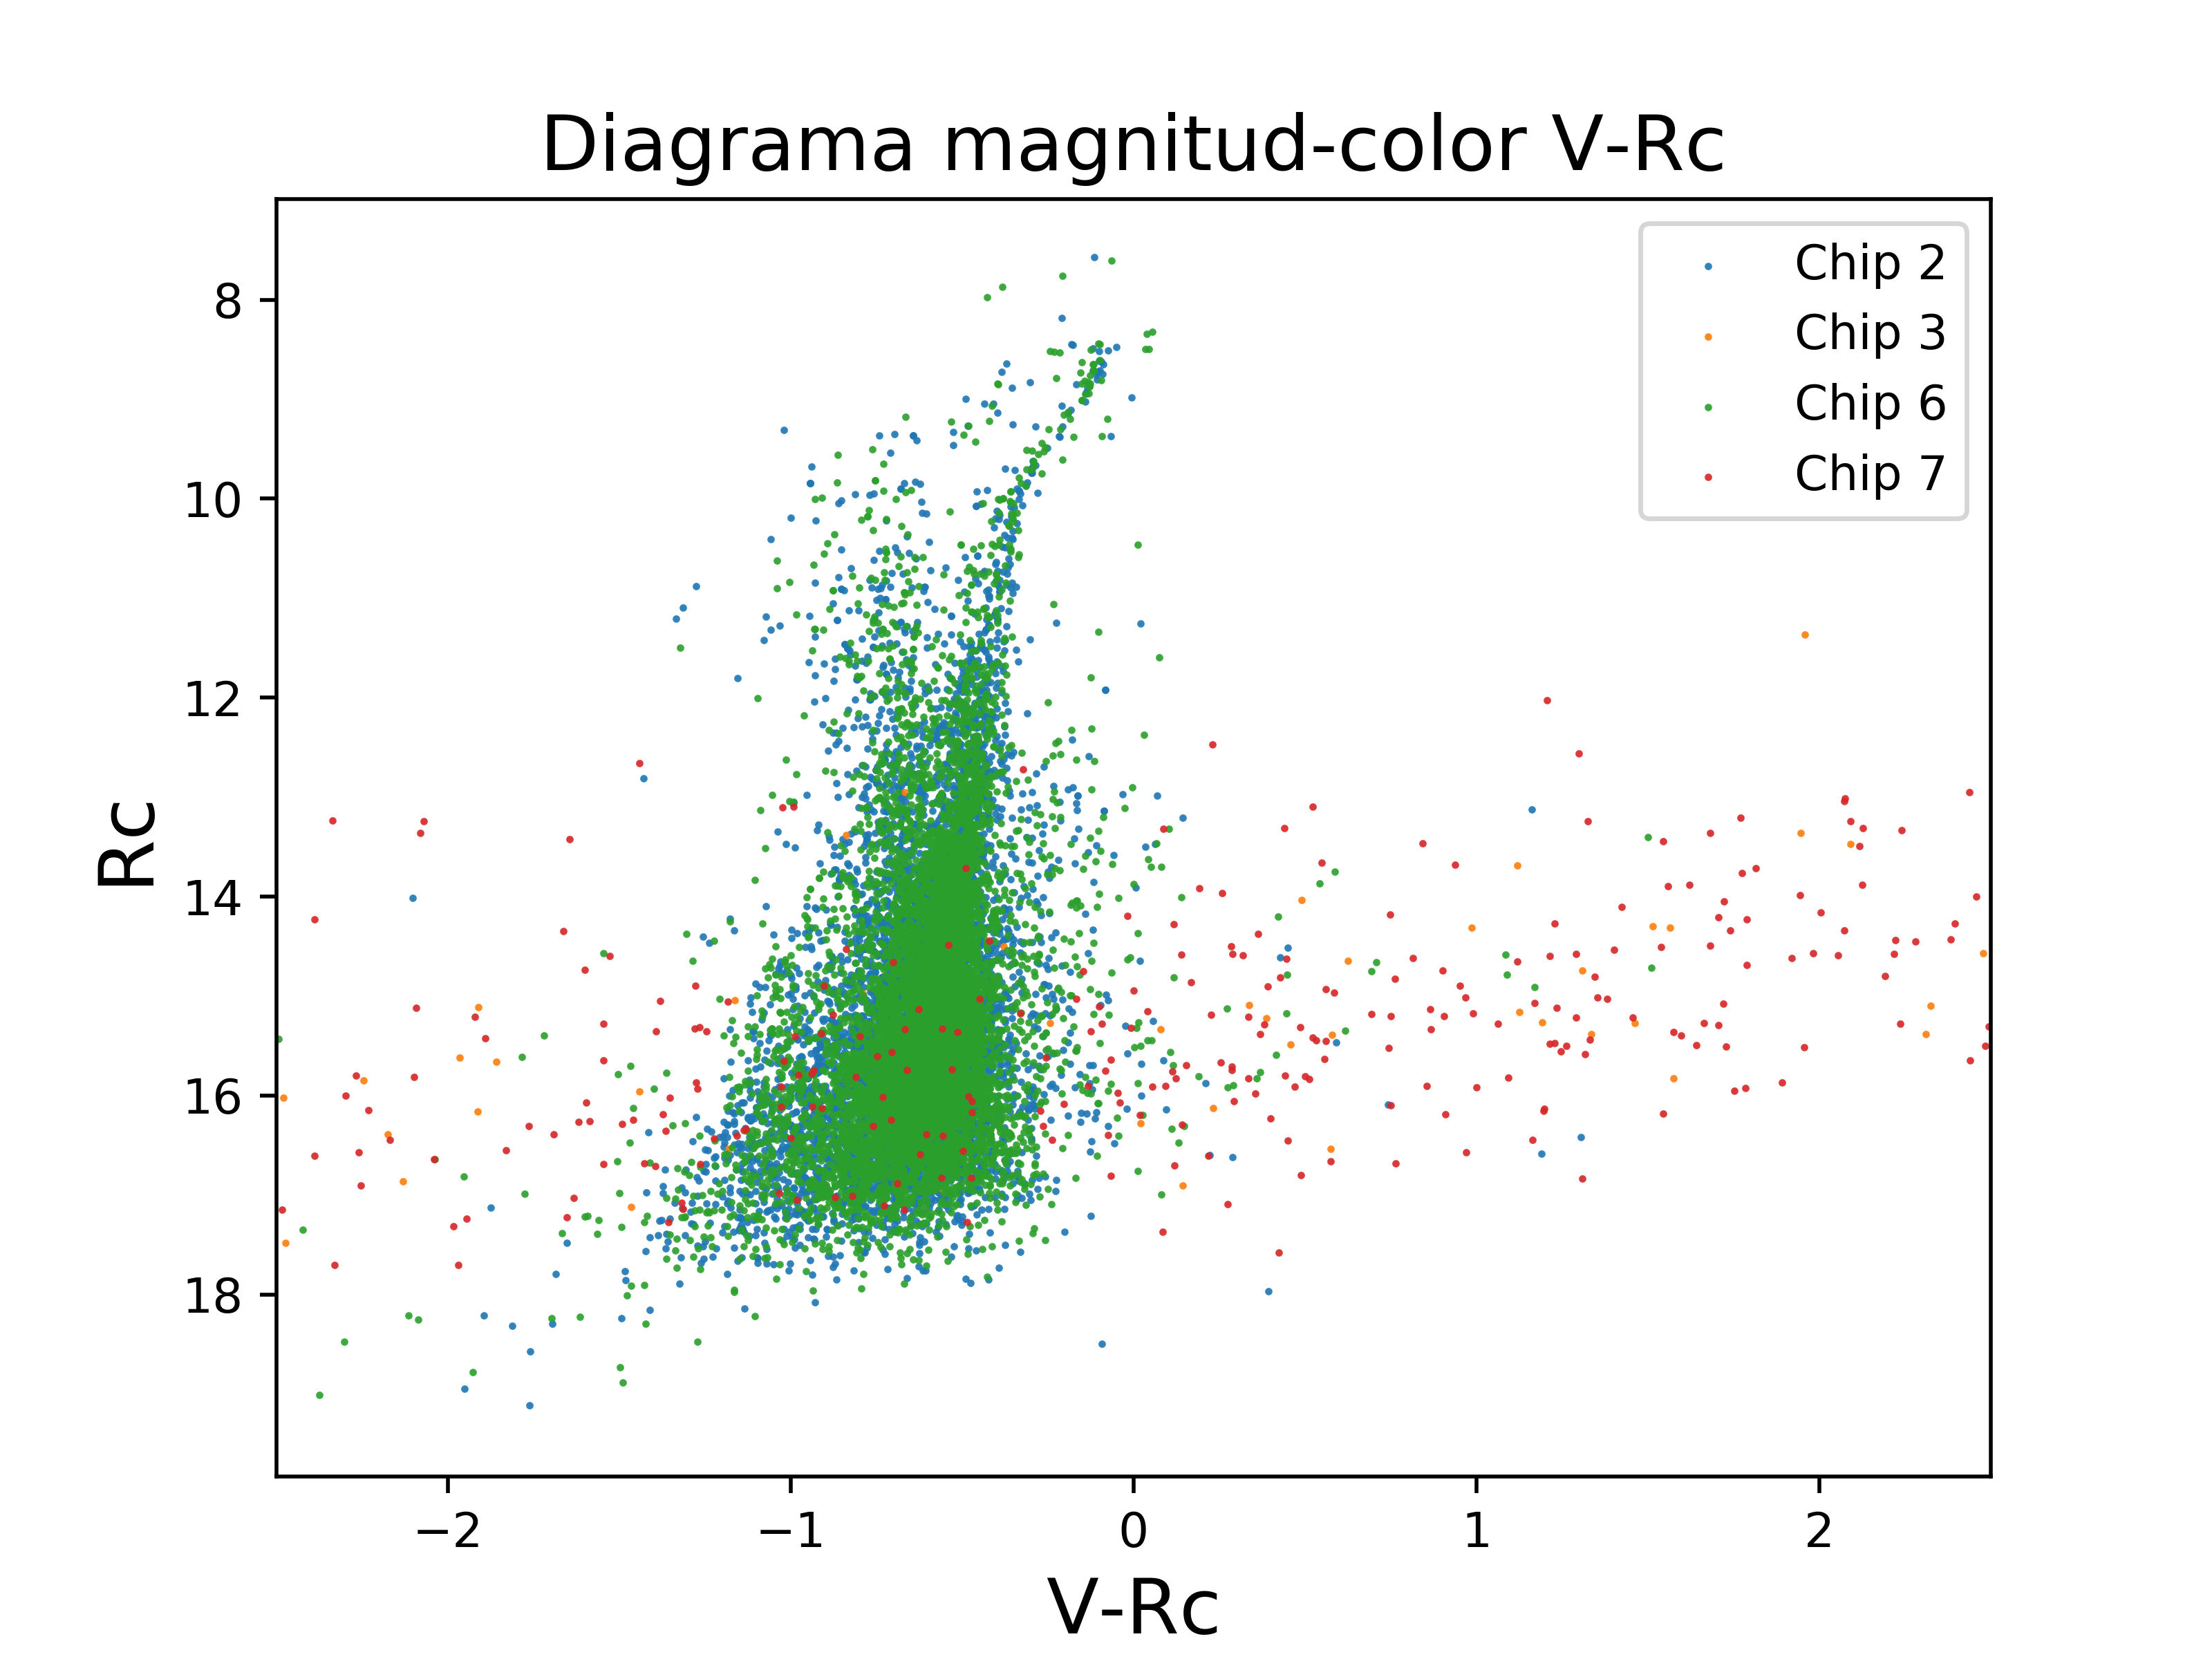
\includegraphics[width = 4in]{diagramaMagnitudColor2.png}
\end{figure}
   

En ambos diagramas se puede apreciar una secuencia principal y una fuerte aglomeración debajo de la secuencia principal. La aglomeración corresponde a estrellas binarias eclipsadas en algún grado por su compañera, o principalmente a enanas blancas. En los diagramas se aprecia interesantemente bien una curva isocrona: la curva pasa por \tqt{el brazo} del lado derecho de las curvas, luego se curva en un pico pronunciado (ese sería el brazo izquierdo) y baja siguiendo la secuencia principal. Las estrellas regadas por fuera de sectores del diagrama corresponden a estrellas atravesadas en el campo y a los chips en donde falló el DAOMATCH y DAOMASTER.



%\bibliography{bibte}
\bibliographystyle{plain}


\end{document}

\begin{figure}[ht!]
  \centering
   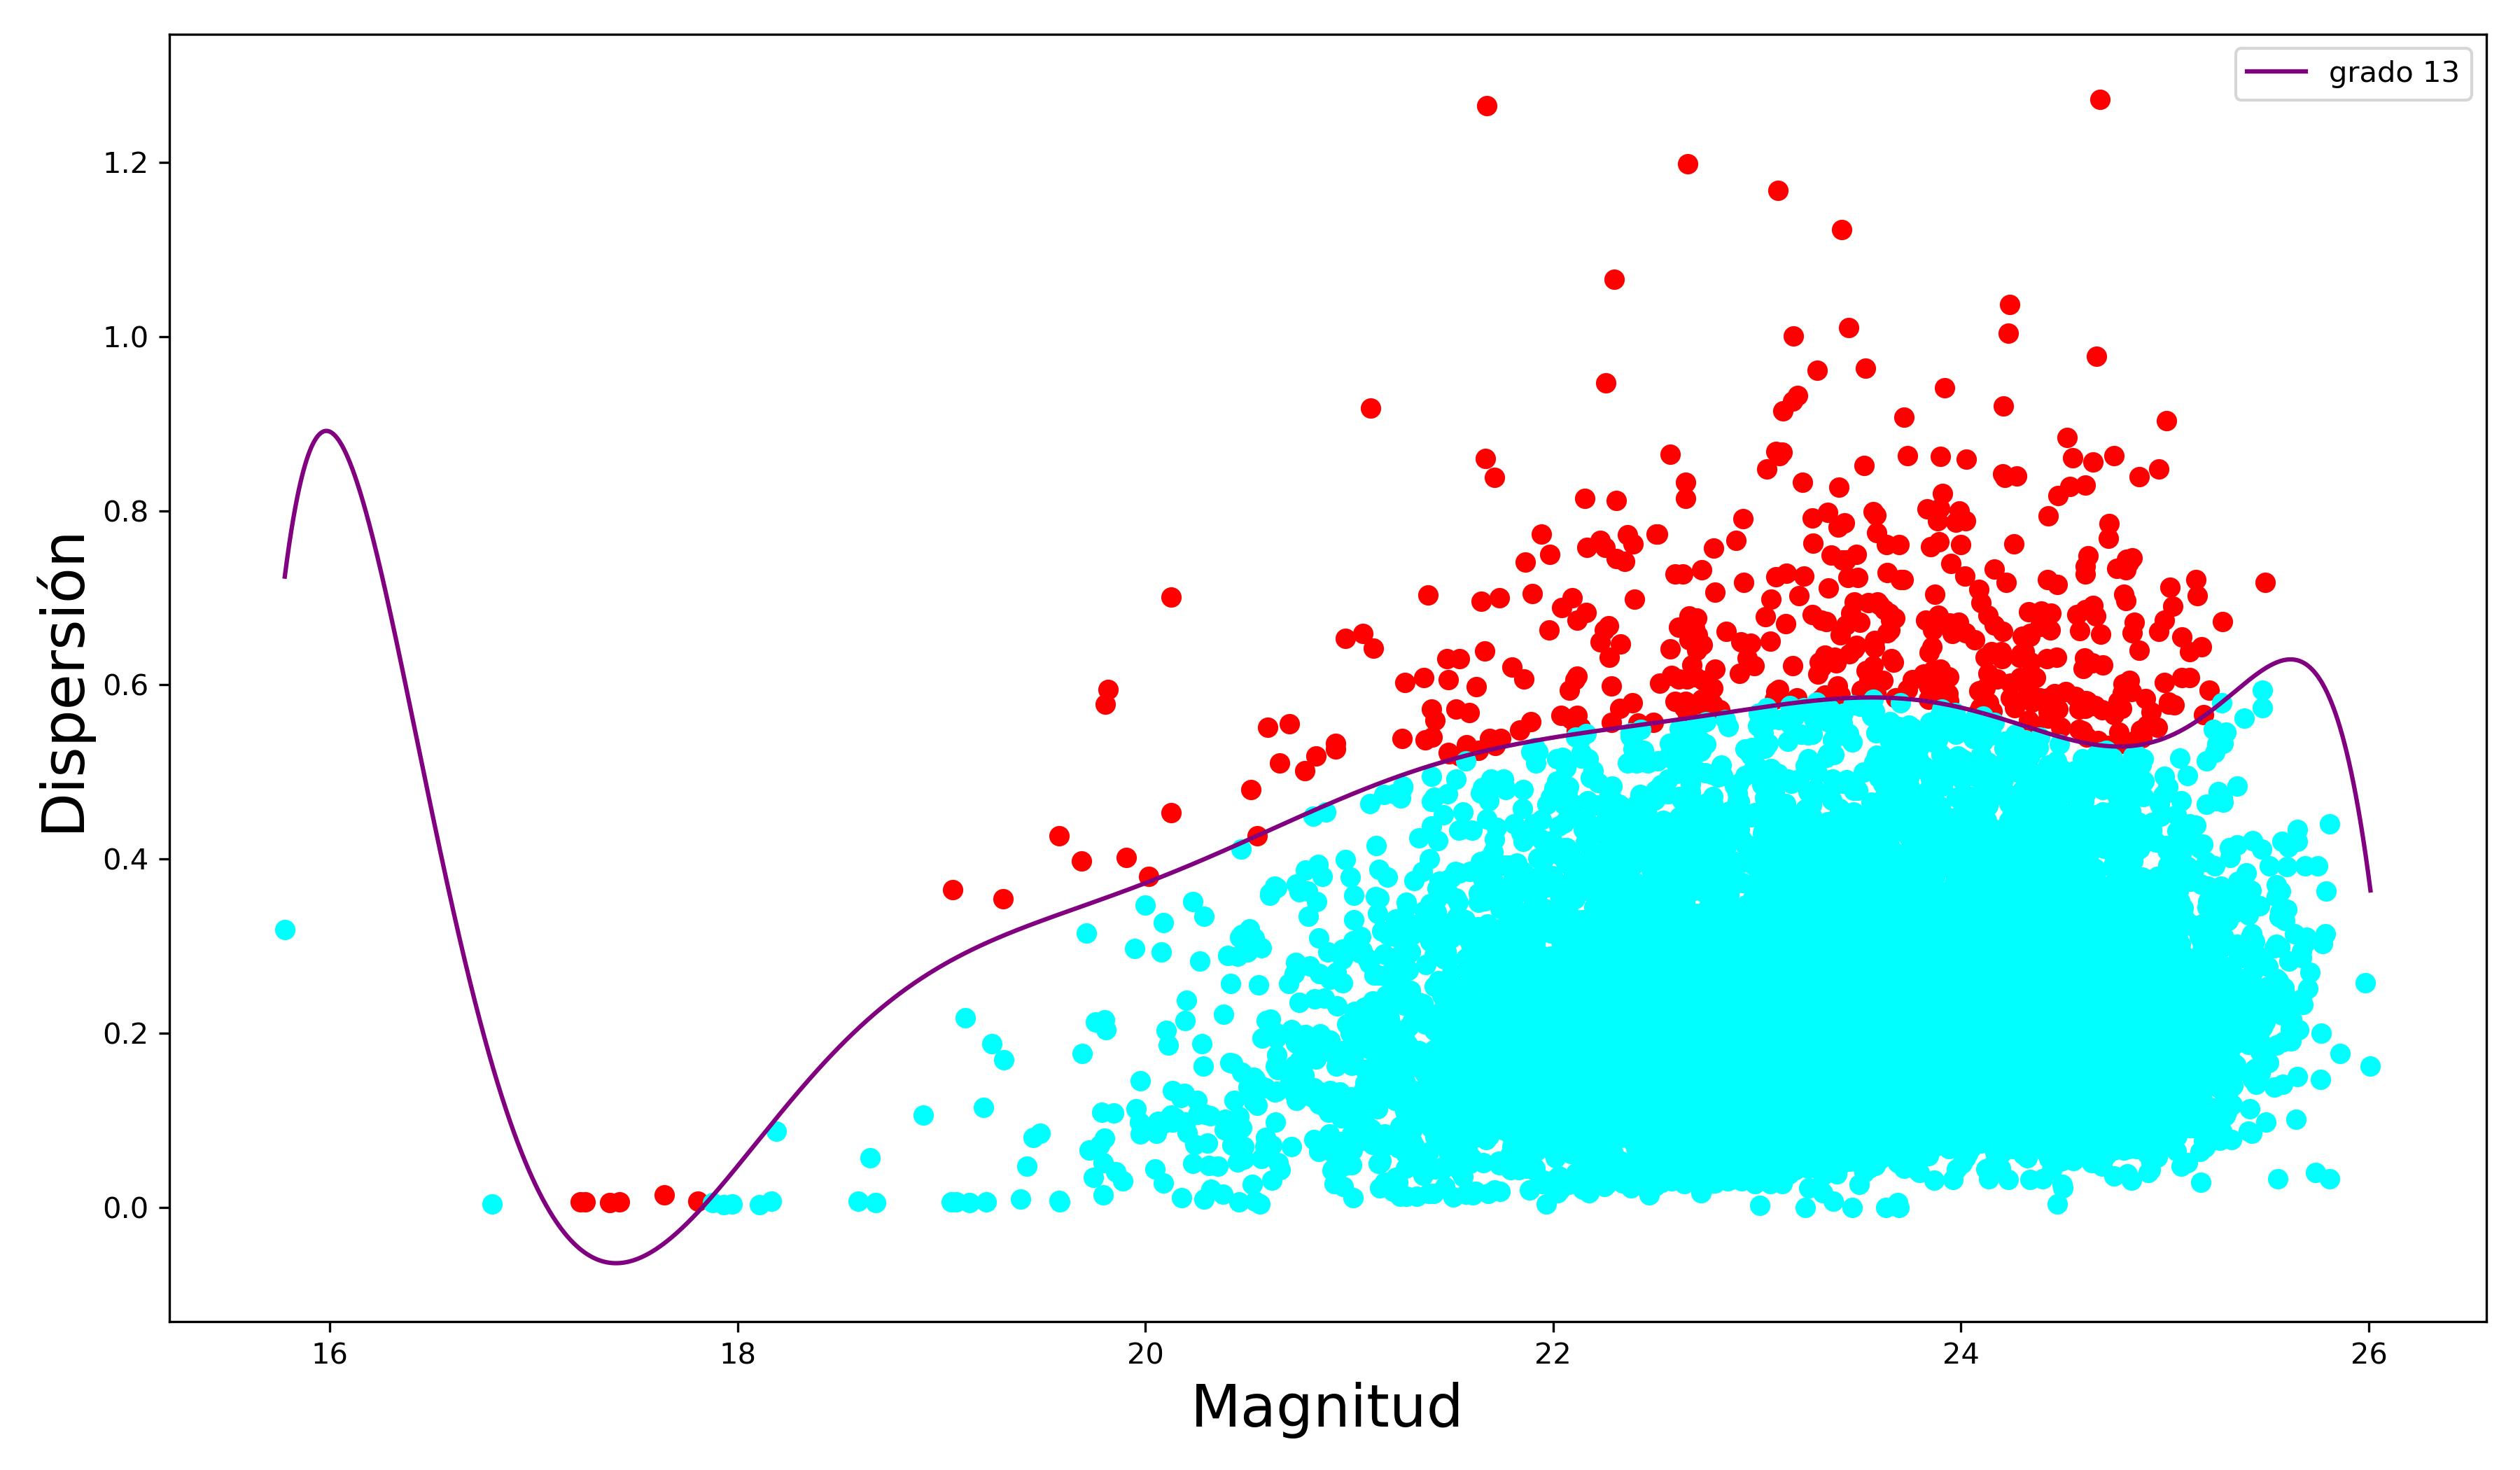
\includegraphics[scale = 0.6]{fits2.png}
  \caption{Estrellas en el espacio de magnitud vs dispersión (usando cantidades robustas) junto a los modelos ya multiplicados por el threshold para buscar candidatos a estrellas variables }
  \label{figura2}
\end{figure}



\begin{figure}[H]
  \centering
   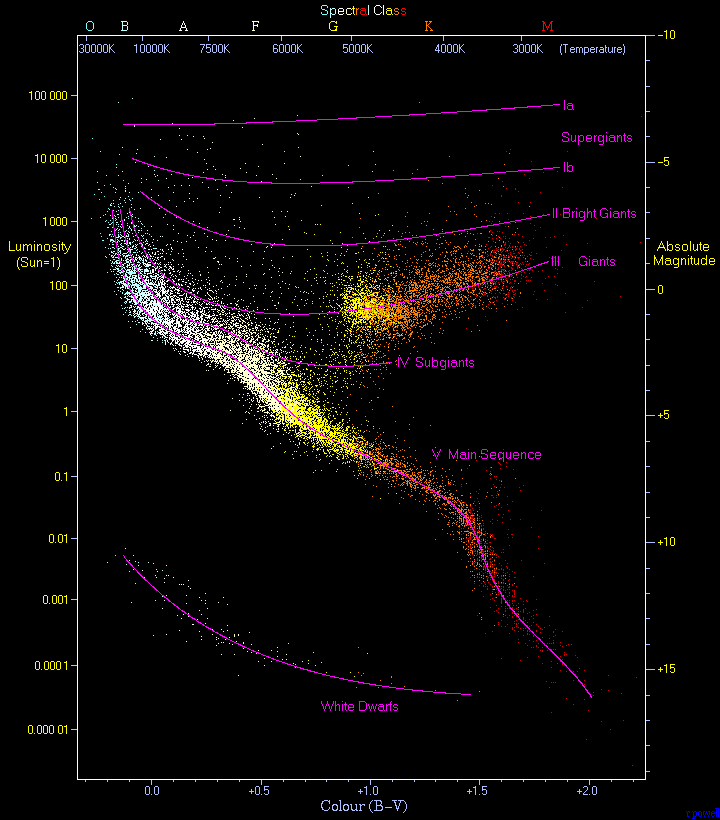
\includegraphics[width= 3.60in]{HRdiag.png}
  %\caption{Diagrama HR de 22000 estrellas del catálogo HIPPARCOS.\cite{hrdiag}  }
  \label{diag}
\end{figure}



\begin{table}[htb]
    \centering
    \label{tabla}
	\begin{tabular}{|c|c|c|c|c| }
	\hline
	Cúmulo & $E(B-V)$ & $m-M$ & Distancia [$pcs$] & Edad del cúmulo [millones de años]  \\ \hline
	NCG 752 & -0.03 & 8.02 & 401.79 & 1259  \\ \hline
	Mel 20 & +0.09 & 6.35 & 186.2 & 63  \\ \hline
	M45 & +0.04 & 5.50 & 125.89 & 126  \\ \hline
	Hyades & 0.00 & 2.84 & 36.98 & 891  \\ \hline
	M44 & +0.04 & 6.21 & 174.58 & 794  \\ \hline
	M67 & -0.03 & 9.32 & 731.14 & 5623  \\ \hline
	IC 4665 & 0.18 & 7.86 & 373.25 & 224  \\ \hline
	M39 & +0.01 & 6.87 & 238.78 & 447  \\ \hline
	\end{tabular}
\end{table}

\begin{table}[htb]
	\begin{tabular}{|c|cccccccccccccccc| }
	\hline
	Tareas $\backslash$ Semanas & 1 & 2 & 3 & 4 & 5 & 6 & 7 & 8 & 9 & 10 & 11 & 12 & 13 & 14 & 15 & 16  \\
	\hline
	1 & X & X & X  &   &   &   &   &  &  &   &   &   &   &   &   &   \\
	2 &   &  & X & X & X &  &  &   &   &  &  &  &   &  &  &   \\
	3 &   &   &   &  & X  & X  & X  & X &   &   &   &  &   &   &  &   \\
	4 &  &  &  &  &  &  &  & X & X & X & X &   &   &   &   &   \\
    5 &  &  &  &  &  &  & X & X &  &  &  &   &   &   &   &   \\
	6 &   &   &   &   &  &   &  X & X  &  &   &  X & X &  X & X  & X &   \\
	\hline
	\end{tabular}
\end{table}
\vspace{1mm}
%CCDRED se encarga de la corrección en sí, sus parámetros son: el tipo de dato de los pixeles (real, short, etc), el nombre del backup (en caso de querer un backup), el archivo de traducción del instrumento (que para una CCD estandar ya viene incluido en IRAF